\let\negmedspace\undefined
\let\negthickspace\undefined
\documentclass[journal,12pt,onecolumn]{IEEEtran}
\usepackage{cite}
\usepackage{amsmath,amssymb,amsfonts,amsthm}
\usepackage{algorithmic}
\usepackage{graphicx}
\usepackage{textcomp}
\usepackage{xcolor}
\usepackage{txfonts}
\usepackage{listings}
\usepackage{enumitem}
\usepackage{mathtools}
\usepackage{gensymb}
\usepackage{comment}
\usepackage[breaklinks=true]{hyperref}
\usepackage{tkz-euclide} 
\usepackage{listings}
\usepackage{gvv}                                        
%\def\inputGnumericTable{}                                 
\usepackage[utf8]{inputenc}
    \usepackage{tfrupee}
\usepackage{xparse}
\usepackage{color}                                            
\usepackage{array}                                            
\usepackage{longtable}                                       
\usepackage{calc}                                             
\usepackage{multirow}
\usepackage{multicol}
\usepackage{hhline}                                           
\usepackage{ifthen}                                           
\usepackage{lscape}
\usepackage{tabularx}
\usepackage{array}
\usepackage{float}
\newtheorem{theorem}{Theorem}[section]
\newtheorem{problem}{Problem}
\newtheorem{proposition}{Proposition}[section]
\newtheorem{lemma}{Lemma}[section]
\newtheorem{corollary}[theorem]{Corollary}
\newtheorem{example}{Example}[section]
\newtheorem{definition}[problem]{Definition}
\newcommand{\BEQA}{\begin{eqnarray}}
\newcommand{\EEQA}{\end{eqnarray}}
\usepackage{float}
%\newcommand{\define}{\stackrel{\triangle}{=}}
\theoremstyle{remark}
\usepackage{ circuitikz }
\begin{document}

\title{2021 XE}
\author{EE25BTECH11021 - Dhanush sagar}
\maketitle
\renewcommand{\thefigure}{\theenumi}
\renewcommand{\thetable}{\theenumi}
\title{2017 Xe}
\author{Dhanush Sagar}
\date{August 2025}



\begin{enumerate}

  \item Gauri said that she can play the keyboard \underline{\hspace{2cm}} her sister. \hfill[GATE XE 2021]

  \begin{multicols}{2}
  \begin{enumerate}
    \item as well as
    \item as better as
    \item as nicest as
    \item as worse as
  \end{enumerate}
  \end{multicols}

  \item A transparent square sheet shown above is folded along the dotted line. The folded sheet will look like \underline{\hspace{1.5cm}}. 
  \begin{figure}[H]
      \centering
      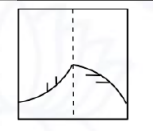
\includegraphics[width=0.3\columnwidth]{figs/fig1.png}
      \caption{}
      \label{fig:placeholder}
  \end{figure}
  
  \hfill[GATE XE 2021]

   \begin{figure}[H]
      \centering
      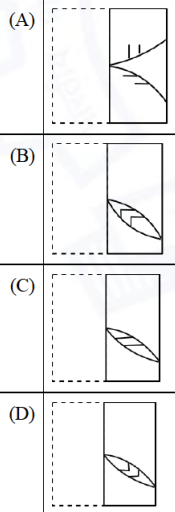
\includegraphics[width=0.3\columnwidth]{figs/fig2.png}
      \caption{}
      \label{fig:placeholder}
  \end{figure}

  \item If $\theta$ is the angle, in degrees, between the longest diagonal of the cube and any one of the edges of the cube, then, $\cos\theta =$ \hfill[GATE XE 2021]

  \begin{multicols}{2}
  \begin{enumerate}
    \item $\dfrac{1}{2}$
    \item $\dfrac{1}{\sqrt{3}}$
    \item $\dfrac{1}{\sqrt{2}}$
    \item $\dfrac{\sqrt{3}}{2}$
  \end{enumerate}
  \end{multicols}

  \item If $\brak{x-\dfrac{1}{2}}^2 - \brak{x-\dfrac{3}{2}}^2 = x+2$, then the value of $x$ is: \hfill[GATE XE 2021]

  \begin{multicols}{2}
  \begin{enumerate}
    \item 2
    \item 4
    \item 6
    \item 8
  \end{enumerate}
  \end{multicols}

  \item \textbf{Pen : Write :: Knife : \underline{\hspace{1.5cm}}}\\
  Which one of the following options maintains a similar logical relation in the above? \hfill[GATE XE 2021]

  \begin{multicols}{2}
  \begin{enumerate}
    \item Vegetables
    \item Sharp
    \item Cut
    \item Blunt
  \end{enumerate}
  \end{multicols}

  \item Listening to music during exercise improves exercise performance and reduces discomfort. Scientists researched whether listening to music while studying can help students learn better and the results were inconclusive. Students who needed external stimulation for studying fared worse while students who did not need any external stimulation benefited from music.\\
  Which one of the following statements is the \textbf{CORRECT} inference of the above passage? \hfill[GATE XE 2021]

  \begin{multicols}{2}
  \begin{enumerate}
    \item Listening to music has no effect on learning and a positive effect on physical exercise.
    \item Listening to music has a clear positive effect both on physical exercise and on learning.
    \item Listening to music has a clear positive effect on physical exercise. Music has a positive effect on learning only in some students.
    \item Listening to music has a clear positive effect on learning in all students. Music has a positive effect only in some students who exercise.
  \end{enumerate}
  \end{multicols}

  \item A jigsaw puzzle has 2 pieces. One of the pieces is shown above. Which one of the given options for the missing piece when assembled will form a rectangle? The piece can be moved, rotated or flipped to assemble with the above piece. 
\begin{figure}[H]
      \centering
      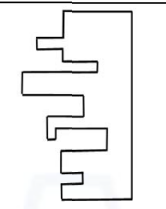
\includegraphics[width=0.2\columnwidth]{figs/fig3.png}
      \caption{}
      \label{fig:placeholder}
  \end{figure}
  
  \hfill[GATE XE 2021]

 \begin{figure}[H]
      \centering
      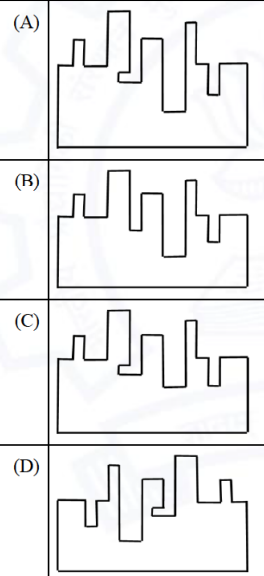
\includegraphics[width=0.3\columnwidth]{figs/fig4.png}
      \caption{}
      \label{fig:placeholder}
  \end{figure}

  \item The number of students in three classes is in the ratio $3:13:6$. If 18 students are added to each class, the ratio changes to $15:35:21$.\\
  The total number of students in all the three classes in the beginning was: \hfill[GATE XE 2021]

  \begin{multicols}{2}
  \begin{enumerate}
    \item 22
    \item 66
    \item 88
    \item 110
  \end{enumerate}
  \end{multicols}

  \item The number of units of a product sold in three different years and the respective net profits are presented in the figure above. The cost/unit in Year 3 was $\rupee{}1$, which was half the cost/unit in Year 2. The cost/unit in Year 3 was one-third of the cost/unit in Year 1. Taxes were paid on the selling price at 10\%, 13\% and 15\% respectively for the three years. Net profit is calculated as the difference between the selling price and the sum of cost and taxes paid in that year.\\
  The ratio of the selling price in Year 2 to the selling price in Year 3 is \underline{\hspace{1.5cm}}. 
  \begin{figure}[H]
      \centering
      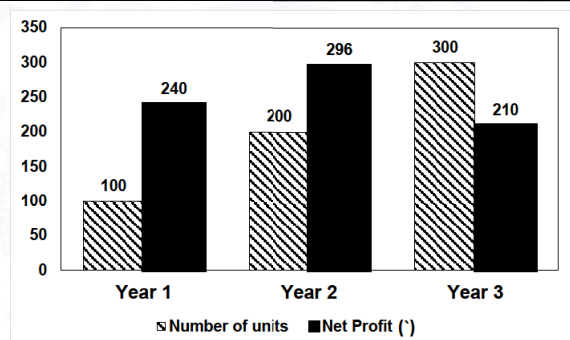
\includegraphics[width=0.5\columnwidth]{figs/fig5.png}
      \caption{}
      \label{fig:placeholder}
  \end{figure}
  
  \hfill[GATE XE 2021]

  \begin{multicols}{2}
  \begin{enumerate}
    \item $4:3$
    \item $1:1$
    \item $3:4$
    \item $1:2$
  \end{enumerate}
  \end{multicols}

  \item Six students P, Q, R, S, T and U, with distinct heights, compare their heights and make the following observations.\\
  \textbf{Observation I:} S is taller than R.\\
  \textbf{Observation II:} Q is the shortest of all.\\
  \textbf{Observation III:} U is taller than only one student.\\
  \textbf{Observation IV:} T is taller than S but is not the tallest.\\
  The number of students that are taller than R is the same as the number of students shorter than \underline{\hspace{1.5cm}}. \hfill[GATE XE 2021]

  \begin{multicols}{2}
  \begin{enumerate}
    \item T
    \item R
    \item S
    \item P
  \end{enumerate}
  \end{multicols}
\item Let
\begin{align}
    S=\brak{AX:\; A=\myvec{2&-4\\[2pt]1&1\\[2pt]1&-1}\ \text{and}\ X=\myvec{x_1\\[2pt]x_2}}.
\end{align}
If \(\myvec{-1\\ \alpha\\ 1}\in S\), then the value of \(\alpha\) is

\hfill[GATE XE 2021]

\begin{multicols}{2}
\begin{enumerate}
\item $-4$
\item $-2$
\item $2$
\item $4$
\end{enumerate}
\end{multicols}


\item Let \(C\) be the boundary of the region \(R: 0\le x\le \pi,\ 0\le y\le \sin x\) in the \(xy\)-plane and \(\alpha\) be the area of the region \(R\). If \(C\) traverses once in the counter clockwise direction, then the value of the line integral \(\displaystyle \oint_C (2y\,dx+5x\,dy)\) is equal to

\hfill[GATE XE 2021]

\begin{multicols}{2}
\begin{enumerate}
\item \(\alpha\)
\item \(2\alpha\)
\item \(3\alpha\)
\item \(4\alpha\)
\end{enumerate}
\end{multicols}


\item Given that \(i=\sqrt{-1}\). The value of
\begin{align}
    \lim_{z\to e^{\pi i/3}}\frac{z^{3}+1}{z^{4}+z^{2}+1}
\end{align}
is

\hfill[GATE XE 2021]

\begin{multicols}{2}
\begin{enumerate}
\item \(\displaystyle \frac{3}{4}+i\,\frac{\sqrt{3}}{4}\)
\item \(\displaystyle \frac{3}{4}-i\,\frac{\sqrt{3}}{4}\)
\item \(\displaystyle -\frac{3}{4}+i\,\frac{\sqrt{3}}{4}\)
\item \(\displaystyle -\frac{3}{4}-i\,\frac{\sqrt{3}}{4}\)
\end{enumerate}
\end{multicols}


\item Let \(f(x)\) be a non-negative continuous function of real variable \(x\). If the area under the curve \(y=f(x)\) from \(x=0\) to \(x=a\) is \(\displaystyle \frac{a^{2}}{2}+\frac{a}{2}\sin a+\frac{\pi}{2}\cos a-\frac{\pi}{2}\), then the value of \(f\!\brak{\frac{\pi}{2}}\) is \rule{2.5cm}{0.15mm} \textit{(round off to one decimal place).}

\hfill[GATE XE 2021]


\item If the numerical approximation of the value of the integral \(\displaystyle \int_{0}^{4} 2^{\alpha x}\,dx\) using the Trapezoidal rule with two subintervals is \(9\), then the value of the real constant \(\alpha\) is \rule{2.5cm}{0.15mm} \textit{(round off to one decimal place).}

\hfill[GATE XE 2021]


\item Let the transformation \(y(x)=e^{x}v(x)\) reduce the ordinary differential equation
\begin{align}
    x\frac{d^{2}y}{dx^{2}}+2(1-x)\frac{dy}{dx}+(x-2)\,y=0;\quad x>0
\end{align}
to
\begin{align}
\alpha x\frac{d^{2}v}{dx^{2}}+2\beta \frac{dv}{dx}+3\gamma v=0,
\end{align}
where \(\alpha,\beta,\gamma\) are real constants. Then, the arithmetic mean of \(\alpha,\beta,\gamma\) is \rule{2.5cm}{0.15mm} \textit{(round off to three decimal places).}

\hfill[GATE XE 2021]


\item A person, who speaks the truth \(3\) out of \(4\) times, throws a fair dice with six faces and informs that the outcome is \(5\). The probability that the outcome is really \(5\) is \rule{2.5cm}{0.15mm} \textit{(round off to three decimal places).}

\hfill[GATE XE 2021]


\item Let \(f(x,y)=x^{4}+y^{4}-2x^{2}+4xy-2y^{2}+\alpha\) be a real valued function. Then, which one of the following statements is TRUE for all \(\alpha\)?

\hfill[GATE XE 2021]

\begin{multicols}{2}
\begin{enumerate}
\item \((0,0)\) is not a stationary point of \(f\)
\item \(f\) has a local maxima at \((0,0)\)
\item \(f\) has a local minima at \((0,0)\)
\item \(f\) has a saddle point at \((0,0)\)
\end{enumerate}
\end{multicols}


\item Let \(u(x,y)=(x^{2}-y^{2})\,v(x,y)\) be such that both \(u(x,y)\) and \(v(x,y)\) satisfy the Laplace equation in a domain \(\Omega\) of the \(xy\)-plane. Then, which one of the following is TRUE in \(\Omega\)?

\hfill[GATE XE 2021]

\begin{multicols}{2}
\begin{enumerate}
\item \(x\,\dfrac{\partial v}{\partial x}-y\,\dfrac{\partial v}{\partial y}=0\)
\item \(x\,\dfrac{\partial v}{\partial x}+y\,\dfrac{\partial v}{\partial y}=0\)
\item \(x\,\dfrac{\partial v}{\partial y}-y\,\dfrac{\partial v}{\partial x}=0\)
\item \(x\,\dfrac{\partial v}{\partial y}+y\,\dfrac{\partial v}{\partial x}=0\)
\end{enumerate}
\end{multicols}

\item
Let $I$ denote the identity matrix of order $7$, and $A$ be a $7\times 7$ real matrix having characteristic polynomial $C_A(\lambda)=\lambda^{2}(\lambda-1)^{\alpha}(\lambda+2)^{\beta}$, where $\alpha$ and $\beta$ are positive integers. If $A$ is diagonalizable and $\operatorname{rank}(A)=\operatorname{rank}(A+2I)$, then $\operatorname{rank}(A-I)$ is \rule{2.5cm}{0.15mm} \textit{(in integer).}

\hfill[GATE XE 2021]


\item
Let $C_1$ be the line segment from $(0,1)$ to $\brak{\tfrac{4}{5},\tfrac{3}{5}}$, and let $C_2$ be the arc of the circle $x^{2}+y^{2}=1$ from $(0,1)$ to $\brak{\tfrac{4}{5},\tfrac{3}{5}}$. If
\begin{align}
    \alpha=\int_{C_1}\!\brak{\frac{2x}{y}\,\hat{\imath}+\frac{1-x^{2}}{y^{2}}\,\hat{\jmath}}\cdot d\vec{r}
\quad\text{and}\quad
\beta=\int_{C_2}\!\brak{\frac{2x}{y}\,\hat{\imath}+\frac{1-x^{2}}{y^{2}}\,\hat{\jmath}}\cdot d\vec{r},
\end{align}
where $\vec{r}=x\,\hat{\imath}+y\,\hat{\jmath}$, then the value of $\alpha^{2}+\beta^{2}$ is \rule{2.5cm}{0.15mm} \textit{(round off to two decimal places).}

\hfill[GATE XE 2021]


\item The general relationship between shear stress, $\tau$, and the velocity gradient $\brak{\dfrac{du}{dy}}$ for a fluid is given by
$\displaystyle \tau = k \brak{\dfrac{du}{dy}}^{n}$, where $k$ is a constant with appropriate units. The fluid is Newtonian if


\hfill[GATE XE 2021]


\begin{multicols}{2}
\begin{enumerate}
\item $n > 1$
\item $n < 1$
\item $n = 1$
\item $n = 0$
\end{enumerate}
\end{multicols}

\vspace{0.8\baselineskip}

\item Which one of the following options is TRUE?


\hfill[GATE XE 2021]


\begin{multicols}{2}
\begin{enumerate}
\item Pathlines and streaklines are the same in an unsteady flow, and streamlines are tangential to the local fluid velocity at a point.
\item Streamlines are perpendicular to the local fluid velocity at a point, and streamlines and streaklines are the same in a steady flow.
\item Pathlines and streaklines are the same in an unsteady flow, and streamlines and streaklines are the same in a steady flow.
\item Streamlines are tangential to the local fluid velocity at a point, and streamlines and streaklines are the same in a steady flow.
\end{enumerate}
\end{multicols}

\vspace{0.8\baselineskip}

\item If $P_{\text{in}}=1.2\ \text{Pa}$ and $P_{\text{out}}=1.0\ \text{Pa}$ are the average pressures at inlet and outlet respectively for a fully-developed flow inside a channel having a height of $50\ \text{cm}$, then the absolute value of average shear stress (in Pa) acting on the walls of the channel of length $5\ \text{m}$ is


\hfill[GATE XE 2021]


\begin{multicols}{2}
\begin{enumerate}
\item 0.005
\item 0.02
\item 0.01
\item 0.05
\end{enumerate}
\end{multicols}

\vspace{0.8\baselineskip}

\item Consider the fully-developed flow of a Newtonian fluid (density $\rho$; viscosity $\mu$) through a smooth pipe of diameter $D$ and length $L$. The average velocity of the flow is $V$. If the length of the pipe is doubled, keeping $V, D, \rho, \mu$ constant, the friction factor


\hfill[GATE XE 2021]


\begin{multicols}{2}
\begin{enumerate}
\item increases by two times
\item remains the same
\item decreases by two times
\item increases by four times
\end{enumerate}
\end{multicols}

\vspace{0.8\baselineskip}

\item The absolute value of pressure difference between the inside and outside of a spherical soap bubble of radius, $R$, and surface tension, $\gamma$, is:


\hfill[GATE XE 2021]


\begin{multicols}{2}
\begin{enumerate}
\item $\dfrac{2\gamma}{R}$
\item $\dfrac{\gamma}{R}$
\item $\dfrac{\gamma}{2R}$
\item $\dfrac{4\gamma}{R}$
\end{enumerate}
\end{multicols}

\vspace{0.8\baselineskip}

\item Which one of the following statements is TRUE about the continuity equation
$\displaystyle \frac{\partial u}{\partial x}+\frac{\partial v}{\partial y}+\frac{\partial w}{\partial z}=0$
(where $u, v, w$ are the velocity components along the $x, y,$ and $z$ coordinates respectively):


\hfill[GATE XE 2021]


\begin{multicols}{2}
\begin{enumerate}
\item The equation is valid only for steady incompressible flows.
\item The equation is valid for both steady and unsteady incompressible flows.
\item The equation is valid only for steady compressible flows.
\item The equation is valid only for unsteady compressible flows.
\end{enumerate}
\end{multicols}

\vspace{0.8\baselineskip}

\item The head loss ($K_L$) associated with the flow entry of water to an internal passage depends on the shape of the entry. The following figure shows three different types of flow entry into a pipe. Which one of the following relationships correctly represents the head loss associated with the three different flow entries?
\begin{figure}[H]
      \centering
      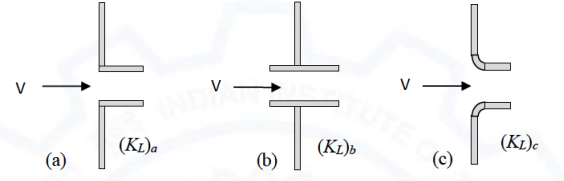
\includegraphics[width=0.5\columnwidth]{figs/fig6.png}
      \caption{}
      \label{fig:placeholder}
  \end{figure}

\hfill[GATE XE 2021]


\begin{multicols}{2}
\begin{enumerate}
\item $(K_L)_a > (K_L)_b > (K_L)_c$
\item $(K_L)_b > (K_L)_a > (K_L)_c$
\item $(K_L)_b \le (K_L)_a = (K_L)_c$
\item $(K_L)_b < (K_L)_a < (K_L)_c$
\end{enumerate}
\end{multicols}

\vspace{0.8\baselineskip}

\item The form and friction drags together contribute to the total drag when flow of air occurs past any object. Two orientations of a finite flat plate are shown in the figure. In Orientation-1, the plate is placed perpendicular to the flow while in Orientation-2, the plate is placed parallel to the flow. If the velocity ($V$) of air in both orientations is the same, which one of the following options is TRUE?
\begin{figure}[H]
      \centering
      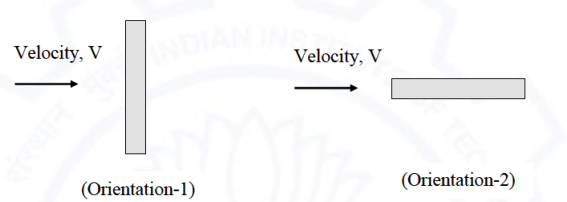
\includegraphics[width=0.6\columnwidth]{figs/fig7.png}
      \caption{}
      \label{fig:placeholder}
  \end{figure}

\hfill[GATE XE 2021]



\begin{enumerate}
\item Orientation-1 has higher form drag and lower friction drag and Orientation-2 has lower form drag and higher friction drag
\item Orientation-1 has lower form drag and lower friction drag and Orientation-2 has higher form drag and higher friction drag
\item Orientation-1 has lower form drag and higher friction drag and Orientation-2 has higher form drag and lower friction drag
\item Orientation-1 has higher form drag and higher friction drag and Orientation-2 has lower form drag and lower friction drag
\end{enumerate}


\item A spherical ball is steadily supported against gravity by an upward air jet as shown in the figure. Take acceleration due to gravity to be $g=10\ \text{m/s}^2$. The mass flow rate of air, reaching the ball, is $0.01\ \text{kg/s}$ and the air reaches the ball at an upward velocity of $3\ \text{m/s}$. Neglecting the buoyancy force, and using the principle of integral momentum balance, the mass (in grams, up to one decimal place) of the ball is \underline{\hspace{2cm}}.

\begin{figure}[H]
      \centering
      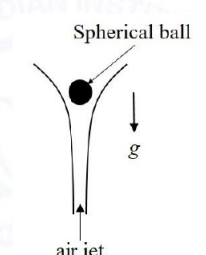
\includegraphics[width=0.4\columnwidth]{figs/fig8.png}
      \caption{}
      \label{fig:placeholder}
  \end{figure}

\hfill[GATE XE 2021]


\item The incompressible flow of air over a curved surface having possible flow separation is schematically shown in the figure. Two zones $P$ and $Q$ are indicated in the figure. Which one of the following combinations is TRUE for zones $P$ and $Q$? \\
(a) Acceleration of flow, (b) Deceleration of flow, (c) Adverse pressure gradient, (d) Favourable pressure gradient, (e) No flow separation, (f) Possible flow separation.

\hfill[GATE XE 2021]

\begin{figure}[H]
      \centering
      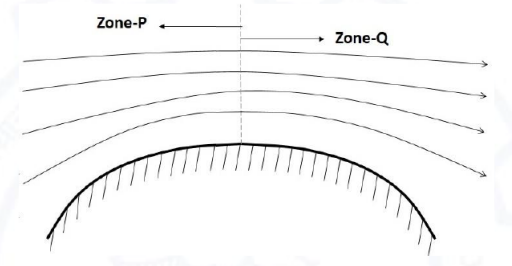
\includegraphics[width=0.6\columnwidth]{figs/fig9.png}
      \caption{}
      \label{fig:placeholder}
  \end{figure}
  
\begin{multicols}{2}
\begin{enumerate}
\item $P$: (a), (d), (e) and $Q$: (b), (c), (f)
\item $P$: (a), (d), (f) and $Q$: (b), (d), (f)
\item $P$: (a), (c), (f) and $Q$: (a), (d), (e)
\item $P$: (a), (c), (e) and $Q$: (a), (d), (f)
\end{enumerate}
\end{multicols}


\item A spherical metal ball (of density $\rho_s$ and diameter $D$), attached to a string, is exposed to a crossflow (of velocity $U_\infty$) of a viscous fluid (of viscosity $\mu$ and density $\rho_f$). Due to the crossflow, the string makes an angle of inclination, $\theta$, with the top surface as shown in the figure. The acceleration due to gravity is denoted by $g$. For this flow, Reynolds number $\displaystyle \mathrm{Re}=\frac{\rho_f U_\infty D}{\mu}\ll 1$ and buoyancy force in the fluid is negligible compared to viscous force. Assuming the string to be weightless and offering negligible drag, the expression for $\theta$ is

\begin{figure}[H]
      \centering
      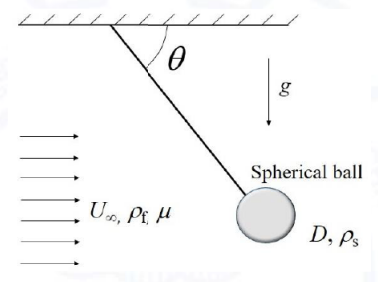
\includegraphics[width=0.5\columnwidth]{figs/fig10.png}
      \caption{}
      \label{fig:placeholder}
  \end{figure}

\hfill[GATE XE 2021]

\begin{multicols}{2}
\begin{enumerate}
\item $\displaystyle \tan\theta=\left[\frac{\rho_s-\rho_f}{18}\,\frac{gD^2}{\mu U_\infty}\right]$
\item $\displaystyle \tan\theta=\left[\frac{1}{18}\,\frac{\rho_f gD^2}{\mu U_\infty}\right]$
\item $\displaystyle \sin\theta=\left[\frac{1}{9}\,\frac{\rho_s gD^2}{\mu U_\infty}\right]$
\item $\displaystyle \tan\theta=\left[\frac{1}{18}\,\frac{\rho_s gD^2}{\mu U_\infty}\right]$
\end{enumerate}
\end{multicols}


\item In a Cartesian coordinate system, a steady, incompressible velocity field of a Newtonian fluid is given by $\mathbf{V}=u_0\!\brak{1-a y^2}\,\mathbf{i}$. Here, $\mathbf{V}$ is the velocity vector in m/s, $\mathbf{i}$ is the unit vector in the $x$–direction, $u_0$ is a positive, real constant (in m/s), and $a$ is a positive, real constant (in m$^{-2}$). The viscosity of the fluid is $\mu$ (in Pa·s). The absolute value of the pressure gradient (in Pa/m) is

\hfill[GATE XE 2021]

\begin{multicols}{2}
\begin{enumerate}
\item $a\,u_0\,\mu$
\item $2a\,u_0\,\mu$
\item $3a\,u_0\,\mu$
\item $4a\,u_0\,\mu$
\end{enumerate}
\end{multicols}


\item In a laminar, incompressible, fully-developed pipe flow of a Newtonian fluid, as shown in the figure, the velocity profile over a cross-section is given by $u=U\!\brak{1-\dfrac{r^2}{R^2}}$, where $U$ is a constant. The pipe length is $L$ and the fluid viscosity is $\mu$. The power $P$ required to sustain the flow is expressed as $P=c\,\mu L U^2$, where $c$ is a dimensionless constant. The value of the constant $c$ (up to one decimal place) is \underline{\hspace{2cm}}.

\begin{figure}[H]
      \centering
      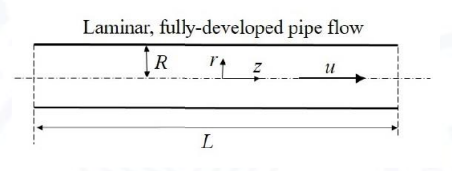
\includegraphics[width=0.5\columnwidth]{figs/fig11.png}
      \caption{}
      \label{fig:placeholder}
  \end{figure}

\hfill[GATE XE 2021]


\item The two-dimensional velocity field $\mathbf{V}$ of a flow in a Cartesian coordinate system is given in dimensionless form by
\begin{align}
\mathbf{V}=\brak{x^2 -a x y}\mathbf{i}+\brak{b x y-\frac{x^2}{2}}\mathbf{j}.
\end{align}
Here, $\mathbf{i}$ and $\mathbf{j}$ are the unit vectors along the $x$ and $y$ directions respectively, $a$ and $b$ are independent of $x$, $y$, and time. If the flow is incompressible, then the value of $(a-b)$, up to one decimal place, is \underline{\hspace{2cm}}.

\hfill[GATE XE 2021]


\item For the configuration shown in the figure, oil of density $800\ \text{kg/m}^3$ lies above water of density $1000\ \text{kg/m}^3$. Assuming hydrostatic conditions and acceleration due to gravity $g=10\ \text{m/s}^2$, the length $L$ (in meters, up to one decimal place) of water in the inclined tube is \underline{\hspace{2cm}}.

\begin{figure}[H]
      \centering
      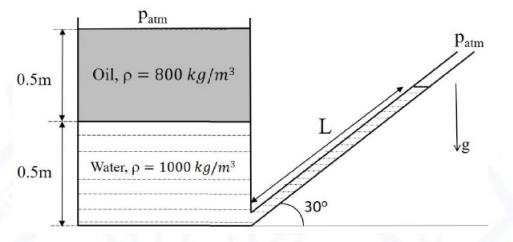
\includegraphics[width=0.5\columnwidth]{figs/fig12.png}
      \caption{}
      \label{fig:placeholder}
  \end{figure}

\hfill[GATE XE 2021]


\item A two-dimensional Eulerian velocity field is given (in m/s) by $\mathbf{V}=[(\sqrt{5})\,x]\mathbf{i}-[(\sqrt{12})\,y]\mathbf{j}$, where $x$ and $y$ are the coordinates (in meters) in a Cartesian coordinate system. The magnitude of the acceleration (in m/s$^2$, up to one decimal place) of a fluid particle at $x=1\ \text{m}$ and $y=-1\ \text{m}$ is \underline{\hspace{2cm}}.

\hfill[GATE XE 2021]


\item A large pump is to deliver oil at an average velocity $(V)$ of $1.5\ \text{m/s}$. The pump has an impeller diameter $(D)$ of $40\ \text{cm}$ and the pressure rise across the pump is $400\ \text{kPa}$. To design this pump, a lab-scale model pump with an impeller diameter of $4\ \text{cm}$ is to be used with water as the fluid. The viscosity $(\mu)$ of the oil is $100$ times that of water, and the densities $(\rho)$ of oil and water are identical. A complete geometric similarity is maintained between the model and prototype. If the pressure rise is a function only of $V$, $D$, $\rho$ and $\mu$, the pressure rise (in kPa, up to one decimal place) across the model pump is \underline{\hspace{2cm}}.

\hfill[GATE XE 2021]


\item Water (density $=10^3\ \text{kg/m}^3$) enters steadily into a horizontal pipe bend, which is part of a larger piping system, as shown in the figure. The volumetric flow rate of water is $0.1\ \text{m}^3/\text{s}$. The gage pressure at the inlet is $500\ \text{kPa}$, while the exit is open to atmosphere. The $x$–component of the force on the support is $F_x$. The absolute value of $F_x$ (in kN, up to one decimal place) is \underline{\hspace{2cm}}.

\begin{figure}[H]
      \centering
      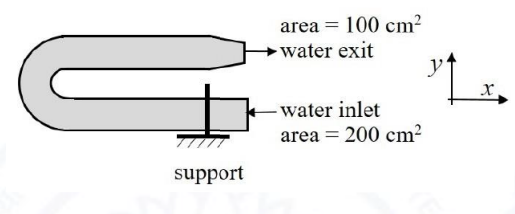
\includegraphics[width=0.5\columnwidth]{figs/fig13.png}
      \caption{}
      \label{fig:placeholder}
  \end{figure}

\hfill[GATE XE 2021]


\item Air (of density $0.5\ \text{kg/m}^3$) enters horizontally into a jet engine at a steady speed of $200\ \text{m/s}$ through an inlet area of $1.0\ \text{m}^2$. Upon entering the engine, the air passes through the combustion chamber and the exhaust gas exits the jet engine horizontally at a constant speed of $700\ \text{m/s}$. The fuel mass flow rate added in the combustion chamber is negligible compared to the air mass flow rate. Also neglect the pressure difference between the inlet air and the exhaust gas. The absolute value of the horizontal force (in kN, up to one decimal place) on the jet engine is \underline{\hspace{2cm}}.

\hfill[GATE XE 2021]


\item Water discharges from a cylindrical tank through an orifice, as shown in the figure. The flow is considered frictionless. Initially, the water level in the tank was $h_1=2\ \text{m}$. The diameter of the tank is $D=1\ \text{m}$, while the diameter of the jet is $d=10\ \text{cm}$, and the acceleration due to gravity is $g=10\ \text{m/s}^2$. The time taken (in seconds, up to one decimal place) for the water level in the tank to come down to $h_2=1\ \text{m}$ is \underline{\hspace{2cm}}.

\begin{figure}[H]
      \centering
      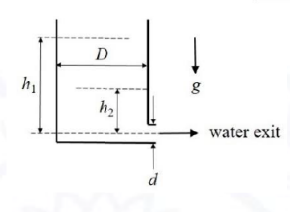
\includegraphics[width=0.5\columnwidth]{figs/fig14.png}
      \caption{}
      \label{fig:placeholder}
  \end{figure}

\hfill[GATE XE 2021]


\item Water discharges steadily from a large reservoir through a long pipeline, as shown in the figure. The Darcy friction factor in the pipe is $0.02$. The pipe diameter is $20\ \text{cm}$ and the discharge of water is $360\ \text{m}^3/\text{h}$. Water level in the reservoir is $10\ \text{m}$ and acceleration due to gravity $g=10\ \text{m/s}^2$. If minor losses are negligible, the length $L$ (in meters, up to one decimal place) of the pipeline is \underline{\hspace{2cm}}.

\begin{figure}[H]
      \centering
      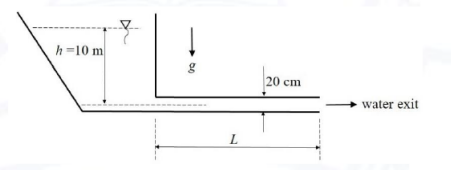
\includegraphics[width=0.5\columnwidth]{figs/fig15.png}
      \caption{}
      \label{fig:placeholder}
  \end{figure}

\hfill[GATE XE 2021]


\item Water is flowing with a flow rate $Q$ in a horizontal circular pipe. Due to the low pressure created at the venturi section (Section–1 in the figure), water from a reservoir is drawn upward using a connecting pipe as shown in the figure. Take acceleration due to gravity $g=10\ \text{m/s}^2$. The flow rate $Q=0.1\ \text{m}^3/\text{s}$, $D_1=8\ \text{cm}$, and $D_2=20\ \text{cm}$. The maximum height $(h$, in meters, up to one decimal place) of the venturi from the reservoir just sufficient to raise the liquid up to Section–1 is \underline{\hspace{2cm}}.

\begin{figure}[H]
      \centering
      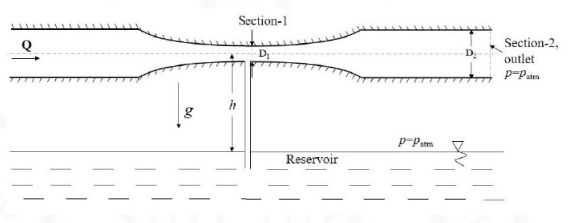
\includegraphics[width=0.5\columnwidth]{figs/fig16.png}
      \caption{}
      \label{fig:placeholder}
  \end{figure}

\hfill[GATE XE 2021]

\item Condition to be satisfied for $\alpha$ and $\beta$ phases to be in equilibrium in a two-component (A and B) system at constant temperature and pressure is (Given: $\mu$ is the chemical potential)

\hfill[GATE XE 2021]

\begin{multicols}{2}
\begin{enumerate}
\item entropy of the system should be maximum
\item Gibbs energy of the system should be minimum and $\mu_A^{\alpha}=\mu_B^{\alpha},\ \mu_A^{\beta}=\mu_B^{\beta}$
\item Gibbs energy of the system should be minimum and $\mu_A^{\alpha}=\mu_A^{\beta},\ \mu_B^{\alpha}=\mu_B^{\beta}$
\item Helmholtz energy should be minimum
\end{enumerate}
\end{multicols}

\item Amino acids react to form peptides and proteins. This process is known as

\hfill[GATE XE 2021]

\begin{multicols}{2}
\begin{enumerate}
\item addition polymerization
\item nucleophilic substitution
\item condensation polymerization
\item hydration
\end{enumerate}
\end{multicols}

\item The most favoured slip system in face centered cubic metal is

\hfill[GATE XE 2021]

\begin{multicols}{2}
\begin{enumerate}
\item $(111)\ [110]$
\item $(110)\ [1\overline{1}1]$
\item $(11\overline{1})\ [112]$
\item $(111)\ [1\overline{1}0]$
\end{enumerate}
\end{multicols}

\item The dielectric constant of a material at ultraviolet frequencies is mainly due to

\hfill[GATE XE 2021]

\begin{multicols}{2}
\begin{enumerate}
\item dipolar polarizability
\item ionic polarizability
\item electronic polarizability
\item interfacial polarizability
\end{enumerate}
\end{multicols}

\item Match the different transformations/reactions in Column I with the most suitable information in Column II. 

\begin{center}
\begin{tabular}{p{6cm} p{6cm}}
\textbf{Column I} & \textbf{Column II} \\
(P) Eutectoid reaction & (1) involves no diffusion \\
(Q) Martensitic transformation & (2) one solid phase transforms into two solid phases \\
(R) Precipitation reaction & (3) occurs in supersaturated solutions \\
\end{tabular}
\end{center}

\hfill[GATE XE 2021]

\begin{multicols}{2}
\begin{enumerate}
\item P–2; Q–3; R–1
\item P–1; Q–2; R–3
\item P–2; Q–1; R–3
\item P–3; Q–2; R–1
\end{enumerate}
\end{multicols}

\item In scanning electron microscopy, the resolution of backscattered electron (BSE) image is poorer compared to that of secondary electron (SE) image, because

\hfill[GATE XE 2021]

\begin{multicols}{2}
\begin{enumerate}
\item energy of BSE is lower
\item sampling volume of BSE is larger
\item yield of BSE is lower
\item sampling volume of SE is larger
\end{enumerate}
\end{multicols}

\item Which of the following deposition conditions favour the formation of larger grains in thin film?

\hfill[GATE XE 2021]

\begin{multicols}{2}
\begin{enumerate}
\item Low deposition rate and low substrate temperature
\item Low deposition rate and high substrate temperature
\item High deposition rate and low substrate temperature
\item High deposition rate and high substrate temperature
\end{enumerate}
\end{multicols}



\item A metal has a melting point of $600^\degree\text{C}$. By rapid cooling, liquid metal can be made to solidify either at $500^\degree\text{C}$ or $400^\degree\text{C}$ or $300^\degree\text{C}$. Critical size of the solid nuclei is

\hfill[GATE XE 2021]

\begin{multicols}{2}
\begin{enumerate}
\item same for solidification at $400^\degree\text{C}$ and $500^\degree\text{C}$
\item smaller for solidification at $400^\degree\text{C}$ as compared to solidification at $500^\degree\text{C}$
\item larger for solidification at $400^\degree\text{C}$ as compared to solidification at $500^\degree\text{C}$
\item the smallest for solidification at $300^\degree\text{C}$
\end{enumerate}
\end{multicols}


\item A magnet of mass $50\ \text{g}$ has a magnetic moment of $4.2\times 10^{-7}\ \text{A}\,\text{m}^2$. The density of the magnet is $7.2\ \text{g}\,\text{cm}^{-3}$. The intensity of magnetization in $\text{A}\,\text{m}^{-1}$ is \underline{\hspace{2cm}} (round off to 3 decimal places).

\hfill[GATE XE 2021]

\end{enumerate}



\begin{enumerate}[resume]

\item In the context of scanning electron microscopy, match the information in Column I with most appropriate information in Column II. 

\begin{center}
\begin{tabular}{p{6cm} p{6cm}}
\textbf{Column I} & \textbf{Column II} \\
(P) Secondary electrons & (1) Crystallographic orientation of grains \\
(Q) Backscattered electrons & (2) Failure analysis of fractured surfaces \\
(R) Characteristic X-rays & (3) Chemical composition analysis \\
(S) Diffracted backscattered electrons & (4) Distinguishing chemically distinct phases \\
\end{tabular}
\end{center}

\hfill[GATE XE 2021]

\begin{multicols}{2}
\begin{enumerate}
\item P–3; Q–2; R–1; S–4
\item P–2; Q–4; R–3; S–1
\item P–1; Q–3; R–2; S–4
\item P–4; Q–2; R–1; S–3
\end{enumerate}
\end{multicols}



\item Match the heat treatment processes given in Column I with the most suitable outcomes in Column II. 

\begin{center}
\begin{tabular}{p{6cm} p{6cm}}
\textbf{Column I} & \textbf{Column II} \\
(P) Quenching & (1) hardens the steel \\
(Q) Annealing & (2) softens the cold worked steel \\
(R) Tempering & (3) toughens the steel \\
(S) Carburizing & (4) hardens the surface of steel \\
\end{tabular}
\end{center}

\hfill[GATE XE 2021]

\begin{multicols}{2}
\begin{enumerate}
\item P–3; Q–2; R–1; S–4
\item P–2; Q–4; R–3; S–1
\item P–1; Q–2; R–3; S–4
\item P–1; Q–3; R–4; S–2
\end{enumerate}
\end{multicols}

\item A co-joined cross-ply laminate composite, as shown in figure, is distorted upon heating. What are the resultant shapes of edges XY and YZ?

\begin{figure}[H]
      \centering
      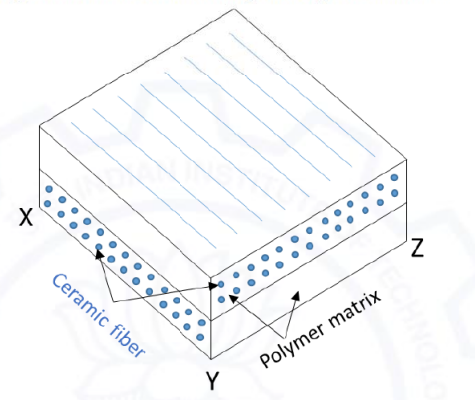
\includegraphics[width=0.5\columnwidth]{figs/fig17.png}
      \caption{}
      \label{fig:placeholder}
  \end{figure}

\hfill[GATE XE 2021]

\begin{multicols}{2}
\begin{enumerate}
\item (A)
\item (B)
\item (C)
\item (D)
\end{enumerate}
\end{multicols}


\item X-ray diffraction peak broadening enables the estimation of

\hfill[GATE XE 2021]

\begin{multicols}{2}
\begin{enumerate}
\item crystallite size of the material
\item microstrain in the material
\item precise lattice parameter
\item residual macrostress acting on the material
\end{enumerate}
\end{multicols}



\item Fe – 10 atom \% C austenite (fcc), having no Fe vacancies, has a lattice parameter of $4\ \text{\AA}$. The density of austenite in $\text{g}\,\text{cm}^{-3}$ is \underline{\hspace{2cm}} (round off to 2 decimal places).\\
(Given: atomic weight of Fe $=55.8$; atomic weight of C $=12.0$; Avogadro’s number $=6.023\times 10^{23}$)

\hfill[GATE XE 2021]

\item An element transforms from $\alpha$ to $\beta$ at $773\ \text{K}$ and $1\ \text{atm}$ pressure with $912\ \text{J mol}^{-1}$ as enthalpy of transformation. The molar volumes of $\alpha$ and $\beta$ phases are $7.377\ \text{cm}^3$ and $7.317\ \text{cm}^3$, respectively. Assume that the difference in molar volumes of $\alpha$ and $\beta$ is independent of pressure. The pressure (in atm) required for $\alpha$ to $\beta$ transformation to occur at $723\ \text{K}$ is \underline{\hspace{2cm}} (round off to nearest integer).\\
(Given: $1\ \text{atm}=1.01325\times 10^{5}\ \text{Pa}$)

\hfill[GATE XE 2021]

\item A binary A–B alloy has $\alpha$ and $\beta$ phases at equilibrium. The ratio of weight percentages (wt.\%) of $\alpha$ to $\beta$ is $4$. The wt.\% of A in $\alpha$ and $\beta$ phases is 70 and 20, respectively. The wt.\% of B in the alloy is \underline{\hspace{2cm}} (round off to nearest integer).

\hfill[GATE XE 2021]

\item During heating, Ti undergoes allotropic transformation from hcp to bcc at $882^\degree\text{C}$. The percent volume change accompanying this transformation is \underline{\hspace{2cm}} (round off to 1 decimal place).\\
(Given: atomic weight of Ti $=47.9$; lattice parameter of bcc Ti $=0.332\ \text{nm}$; density of hcp Ti $=4.51\ \text{g cm}^{-3}$; Avogadro’s number $=6.023\times 10^{23}$)

\hfill[GATE XE 2021]

\item Vickers hardness test is performed with an indenter of square-base diamond pyramid having an included angle of $136^\degree$ between the opposite faces of the pyramid. If the applied load is $10\ \text{kg}$ and the average length of diagonals of square indentation is $0.5\ \text{mm}$, the Vickers hardness in $\text{kg mm}^{-2}$ is \underline{\hspace{2cm}} (round off to nearest integer).

\hfill[GATE XE 2021]

\item The drift mobility of electron in an n-type Si crystal doped with $10^{16}\ \text{cm}^{-3}$ phosphorous atoms is $1350\ \text{cm}^2\,\text{V}^{-1}\,\text{s}^{-1}$. The electrical conductivity in $\Omega^{-1}\,\text{m}^{-1}$ is \underline{\hspace{2cm}} (round off to nearest integer).\\
(Given: Intrinsic charge concentration of Si $=1.45\times 10^{10}\ \text{cm}^{-3}$; Charge of an electron, $e=1.6\times 10^{-19}\ \text{C}$)

\hfill[GATE XE 2021]

\item At $1000\ \text{K}$, the linear thermal expansion coefficients of graphite, parallel and perpendicular to the graphite layers, are $0.8\times 10^{-6}\ \text{K}^{-1}$ and $29\times 10^{-6}\ \text{K}^{-1}$, respectively. The percentage increase in the volume of graphite when heated from $900\ \text{K}$ to $1100\ \text{K}$ is \underline{\hspace{2cm}} (round off to 2 decimal places).

\hfill[GATE XE 2021]

\item A certain ceramic has a theoretical density and sintered density of $6.76\ \text{g cm}^{-3}$ and $6.60\ \text{g cm}^{-3}$, respectively. The green compact has 18 volume percent porosity. For a sintered cube of side $2\ \text{cm}$, the required side of the cubic green compact in cm is \underline{\hspace{2cm}} (round off to 2 decimal places).

\hfill[GATE XE 2021]

\item When a metal (M) is immersed in de-aerated acid electrolyte, it polarizes anodically by $0.4\ \text{V}$. The M/M$^{n+}$ exchange current density is $10^{-5}\ \text{A m}^{-2}$ and Tafel slope is $0.1\ \text{V/decade}$ for the anodic reaction. Assume that corrosion is uniform and, anodic and cathodic reactions are under activation control. The rate of metal dissolution in $\text{A m}^{-2}$ is \underline{\hspace{2cm}} (round off to 1 decimal place).

\hfill[GATE XE 2021]

\item A force $F=40$ kN is applied on the hook as shown. The equivalent force-couple system at $B$ is

\begin{figure}[H]
      \centering
      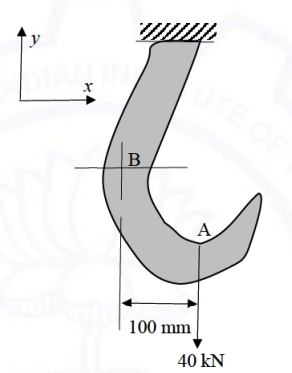
\includegraphics[width=0.4\columnwidth]{figs/fig18.png}
      \caption{}
      \label{fig:placeholder}
  \end{figure}

\hfill[GATE XE 2021]

\begin{multicols}{2}
\begin{enumerate}
\item 40 kN in $+y$ direction and $M=0$
\item 40 kN in $-y$ direction and $M=0$
\item 40 kN in $+y$ direction and $M=4000$ Nm counter clockwise
\item 40 kN in $-y$ direction and $M=4000$ Nm clockwise
\end{enumerate}
\end{multicols}

\item A rigid rod $OA$ rotates clockwise at an angular velocity of 10 rad/s. A bead $B$ ($OB=1$ m) translates outward on the rod at a speed of 5 m/s and acceleration 2.5 m/s$^2$ (both quantities with respect to the rod). The Coriolis component of acceleration is

\begin{figure}[H]
      \centering
      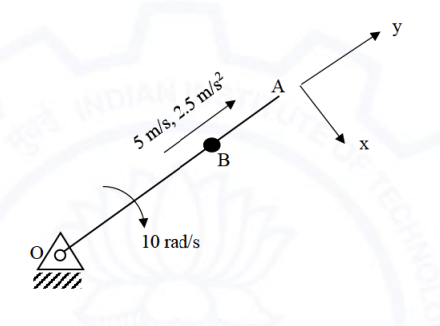
\includegraphics[width=0.5\columnwidth]{figs/fig19.png}
      \caption{}
      \label{fig:placeholder}
  \end{figure}

\hfill[GATE XE 2021]

\begin{multicols}{2}
\begin{enumerate}
\item 2.5 m/s$^2$ in $+x$ direction
\item 100 m/s$^2$ in $+x$ direction
\item 100 m/s$^2$ in $-y$ direction
\item 25 m/s$^2$ in $+y$ direction
\end{enumerate}
\end{multicols}

\item A two force member in equilibrium is one in which

\hfill[GATE XE 2021]

\begin{multicols}{2}
\begin{enumerate}
\item Forces act at two points and forces are collinear
\item Forces act at two points and member is always straight
\item Forces act at two points but the member is free to carry moment at any point
\item Force acts at one point and moment acts at second point
\end{enumerate}
\end{multicols}

\item If the yield point shear stress obtained from the torsion test of a cylindrical specimen is $\tau_y$, then what is the maximum value of principal strain at yielding? ($\mu$ is Poisson’s ratio and $E$ is Young’s modulus)

\hfill[GATE XE 2021]

\begin{multicols}{2}
\begin{enumerate}
\item $\dfrac{\tau_y}{E}$
\item $\dfrac{(1+\mu)\tau_y}{E}$
\item $\dfrac{\tau_y}{2E}$
\item $\dfrac{(1-\mu)\tau_y}{E}$
\end{enumerate}
\end{multicols}

\item If the ratio of Young’s modulus to bulk modulus of a material is $3/2$, then the ratio of shear modulus to the Young’s modulus of the material is

\hfill[GATE XE 2021]

\begin{multicols}{2}
\begin{enumerate}
\item 1
\item 2/5
\item 1/3
\item 3/5
\end{enumerate}
\end{multicols}

\item With respect to the plane of maximum shear stress, which of the following statements is \textbf{INCORRECT}?

\hfill[GATE XE 2021]

\begin{multicols}{2}
\begin{enumerate}
\item The normal stress on this plane is zero.
\item The maximum shear stress is equal to the largest of the one half the difference of principal stresses
\item The plane of maximum shear stress occurs at $45^\degree$ to the principal planes.
\item The magnitude of the maximum shear stress is equal to the largest of the radius of the Mohr’s circles.
\end{enumerate}
\end{multicols}

\item A simply supported beam of length $L$ is loaded by two symmetrically applied point loads $P$ at $L/3$ from each support. Both the loads are then shifted to new points which are at a distance $L/4$ from each support. The bending moments at the mid-section of the beam in both the cases are same. The magnitude of $P_1$ in terms of $P$ is

\begin{figure}[H]
      \centering
      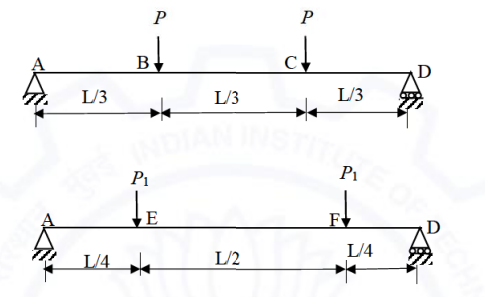
\includegraphics[width=0.5\columnwidth]{figs/fig20.png}
      \caption{}
      \label{fig:placeholder}
  \end{figure}

\hfill[GATE XE 2021]

\begin{multicols}{2}
\begin{enumerate}
\item $P/4$
\item $8P/3$
\item $4P/3$
\item $P/3$
\end{enumerate}
\end{multicols}

\item A beam having rectangular cross section is subjected to transverse loading. The ratio of maximum shear stress developed in the beam to the average shear stress is

\hfill[GATE XE 2021]

\begin{multicols}{2}
\begin{enumerate}
\item 1.50
\item 1.25
\item 1.33
\item 1.66
\end{enumerate}
\end{multicols}

\item During an earthquake, a structure vibrates and the vibration can be assumed to be in simple harmonic motion at 5 Hz. At a measurement point, the RMS value of acceleration is 10 m/s$^2$. The approximate amplitude of motion (in mm) at this point \emph{(rounded off to two decimal places)} is \rule{3cm}{0.4pt}

\hfill[GATE XE 2021]

\item For the state of plane stress shown, the components of normal and shear stresses are given in terms of stress $\sigma$ and unknown constants $m$ and $n$. If the normal and shear components of stress on a $45^\degree$ plane are $2\sigma$ and zero, the values of $m$ and $n$ would be:

\begin{figure}[H]
      \centering
      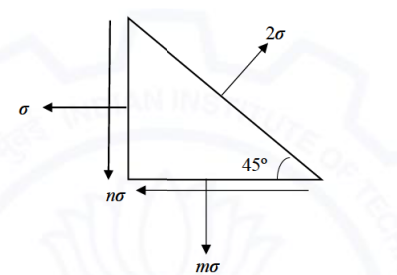
\includegraphics[width=0.5\columnwidth]{figs/fig21.png}
      \caption{}
      \label{fig:placeholder}
  \end{figure}

\hfill[GATE XE 2021]

\begin{multicols}{2}
\begin{enumerate}
\item $m=1,\; n=2$
\item $m=2,\; n=1$
\item $m=1,\; n=1$
\item $m=2,\; n=2$
\end{enumerate}
\end{multicols}

\item For a state of plane strain, the normal strains are given by $\varepsilon_{xx}=1000\times10^{-6}$, $\varepsilon_{yy}=200\times10^{-6}$ and the maximum shear strain is $\gamma_{\max}=1000\times10^{-6}$. The value of shear strain $\gamma_{xy}$ for this strain state is

\hfill[GATE XE 2021]

\begin{multicols}{2}
\begin{enumerate}
\item $600\times10^{-6}$
\item $183\times10^{-6}$
\item $1000\times10^{-6}$
\item $800\times10^{-6}$
\end{enumerate}
\end{multicols}

\item A thin cylinder (closed at its ends) of radius $r$ and thickness $t$ ($r\gg t$) is subjected to internal pressure $p$. The maximum shear stress in the wall of the cylinder is



\hfill[GATE XE 2021]

\begin{multicols}{2}
\begin{enumerate}
\item $\dfrac{pr}{t}$
\item $\dfrac{pr}{2t}$
\item $\dfrac{pr}{4t}$
\item $\dfrac{3pr}{2t}$
\end{enumerate}
\end{multicols}

\item The truss shown is subjected to a force $P$. All members of the truss have the same length $L$. The reaction at $A$ and force in member $AB$ are

\begin{figure}[H]
      \centering
      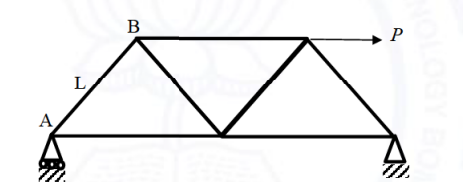
\includegraphics[width=0.5\columnwidth]{figs/fig22.png}
      \caption{}
      \label{fig:placeholder}
  \end{figure}

\hfill[GATE XE 2021]

\begin{multicols}{2}
\begin{enumerate}
\item $\dfrac{P\sqrt{3}}{4}$ \; and \; $\dfrac{P}{2}$
\item $\dfrac{P\sqrt{3}}{8}$ \; and \; $\dfrac{P\sqrt{3}}{4}$
\item $\dfrac{P\sqrt{3}}{4}$ \; and \; $\dfrac{P}{4}$
\item $P$ \; and \; $\dfrac{P}{4}$
\end{enumerate}
\end{multicols}

\item The figure shows a structure with supports. The correct free body diagram when the supports are removed is

\begin{figure}[H]
      \centering
      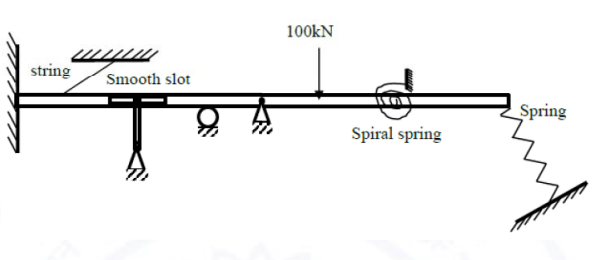
\includegraphics[width=0.5\columnwidth]{figs/fig23.png}
      \caption{}
      \label{fig:placeholder}
  \end{figure}

\hfill[GATE XE 2021]

\begin{figure}[H]
      \centering
      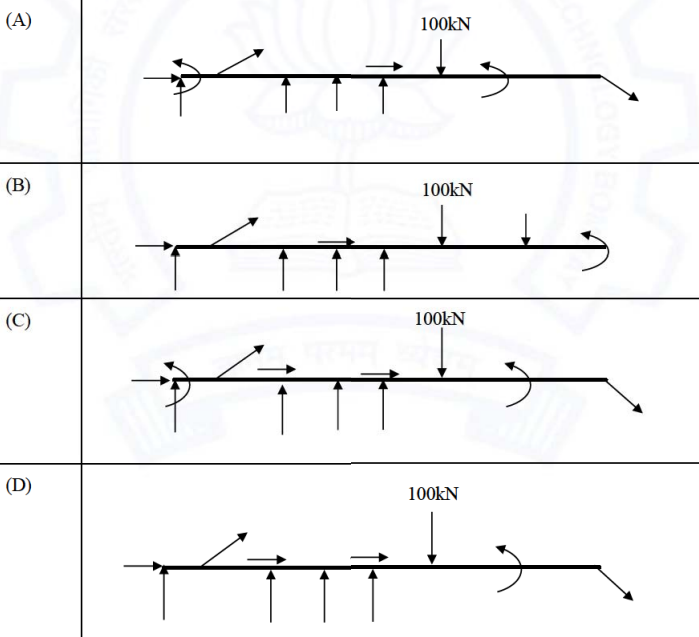
\includegraphics[width=0.5\columnwidth]{figs/fig24.png}
      \caption{}
      \label{fig:placeholder}
  \end{figure}





\item A hammer of mass 1 kg is used to break an almond shell. The velocity–time graph of the hammer during the impact duration is shown in the figure. The shape of force–time graph is also given, which can be approximated as a triangle. A force of 300 N is required for breaking the shell, while a force of 200 N will not be able to break it, but just introduce a crack. Which one of the following events will happen?

\begin{figure}[H]
      \centering
      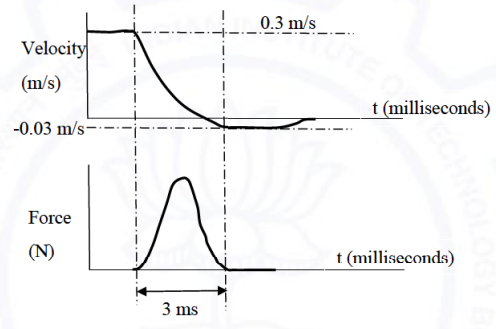
\includegraphics[width=0.5\columnwidth]{figs/fig25.png}
      \caption{}
      \label{fig:placeholder}
  \end{figure}

\hfill[GATE XE 2021]

\begin{multicols}{2}
\begin{enumerate}
\item Shell will crack but not break
\item Shell will break
\item Shell will remain intact
\item Cannot be determined from the given data
\end{enumerate}
\end{multicols}


\item A rigid circular disc of radius 0.2 m and mass 10 kg rolls without slip on the ground at A. The coefficient of static friction between ground and disc is 0.7. A torque $T = 9$ Nm acts on the disc as shown. Given acceleration due to gravity $g = 10\ \text{m/s}^2$. The friction force acting on the disc (in N, integer) is \rule{3cm}{0.15mm}.

\begin{figure}[H]
      \centering
      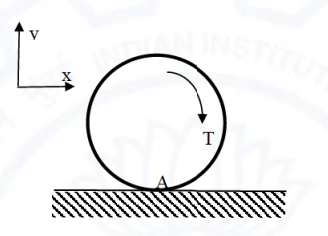
\includegraphics[width=0.5\columnwidth]{figs/fig26.png}
      \caption{}
      \label{fig:placeholder}
  \end{figure}

\hfill[GATE XE 2021]


\item A prismatic solid circular rod of diameter $d$ is bent to introduce an offset $s=d$ as shown. The rod is further subjected to an axial load $P$. If the maximum longitudinal stress at a section A–B in the rod (with offset) is $n$ times the longitudinal stress in the straight rod, the value of $n$ (in integer) would be \rule{3cm}{0.15mm}.

\begin{figure}[H]
      \centering
      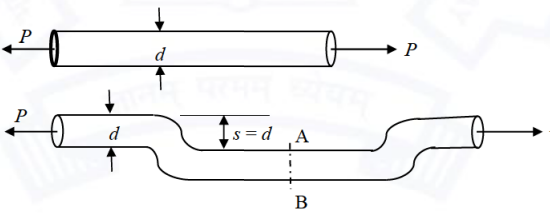
\includegraphics[width=0.5\columnwidth]{figs/fig27.png}
      \caption{}
      \label{fig:placeholder}
  \end{figure}

\hfill[GATE XE 2021]


\item A naturally curved steel beam AB having Young’s modulus $E = 208$ GPa, area moment of inertia $I = 26.7\ \text{cm}^4$ and radius $R = 2$ m is subjected to a vertical load $P = 1000$ N at B. The end A at $\theta = 90^\circ$ is rigidly fixed. The bending strain energy of the beam (in Nm, rounded off to two decimal places) is \rule{3cm}{0.15mm}.

\begin{figure}[H]
      \centering
      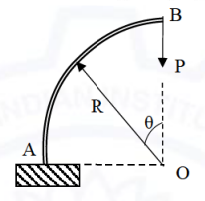
\includegraphics[width=0.4\columnwidth]{figs/fig28.png}
      \caption{}
      \label{fig:placeholder}
  \end{figure}

\hfill[GATE XE 2021]


\item At room temperature of $25^\circ$C, a gap of 1 mm exists between the ends of the rods 1 and 2 as shown. Given the cross-sectional area $A$ of the rods is $1500\ \text{mm}^2$, Young’s modulus $E = 75$ GPa and the coefficient of thermal expansion $\alpha = 23 \times 10^{-6}$/°C. When the temperature has reached $150^\circ$C, the magnitude of normal stress in each of the rods (in MPa, rounded off to two decimal places) is \rule{3cm}{0.15mm}.

\begin{figure}[H]
      \centering
      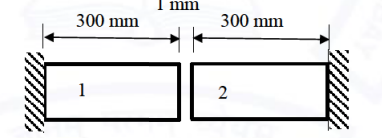
\includegraphics[width=0.5\columnwidth]{figs/fig29.png}
      \caption{}
      \label{fig:placeholder}
  \end{figure}

\hfill[GATE XE 2021]


\item A tube of inner radius 4 cm and outer radius 5 cm can carry a maximum torque $T$. This tube is now replaced by a solid circular shaft of the same material. The minimum radius of the solid circular shaft (in cm, rounded off to two decimal places) to carry the same amount of torque $T$ is \rule{3cm}{0.15mm}.

\hfill[GATE XE 2021]


\item In System A, a rectangular block of mass $M$ is centrally supported on a spring of stiffness $K$ as shown. In System B, the mass is hinged at one of its ends and is supported centrally by the spring. The ratio of natural frequency of System B to that of System A (rounded off to two decimal places) is \rule{3cm}{0.15mm}.

\begin{figure}[H]
      \centering
      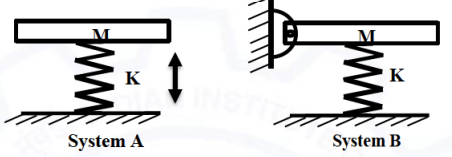
\includegraphics[width=0.5\columnwidth]{figs/fig30.png}
      \caption{}
      \label{fig:placeholder}
  \end{figure}

\hfill[GATE XE 2021]

\item A coronavirus droplet of mass 1 microgram ejects from the mouth of a patient with a velocity of 0.7 m/s and travels through air. The gravitational force experienced by it can be neglected due to the buoyancy effect. However, the droplet experiences air drag force proportional to its velocity and the drag coefficient is given as 1.0 $\mu$N$\cdot$s/m. The distance travelled by the droplet before its velocity drops to 10\% of its initial velocity \emph{(in m, rounded off to two decimal places)} is \rule{3cm}{0.4pt}

\hfill[GATE XE 2021]
\item A refrigerator working on a reversed Carnot cycle has a Coefficient of Performance (COP) of 4. If it works as a heat pump and consumes work input of 1 kW, the heating effect will be:

\hfill[GATE XE 2021]

\begin{multicols}{2}
\begin{enumerate}
\item 1 kW
\item 4 kW
\item 5 kW
\item 6 kW
\end{enumerate}
\end{multicols}


\item The liquid phase of a pure substance is termed as, if its temperature is lower than the saturation temperature corresponding to its pressure $P$.

\hfill[GATE XE 2021]

\begin{multicols}{2}
\begin{enumerate}
\item super-heated liquid
\item sub-cooled liquid
\item metastable liquid
\item flashing liquid
\end{enumerate}
\end{multicols}

\item Two air streams of mass flow rates $\dot{m}_1$ and $\dot{m}_2$ enter a mixing chamber and exit after perfect mixing. The corresponding temperatures of the inlet streams are $T_1$ and $T_2$, respectively. Heat loss rate from the mixing chamber to the surrounding is $\dot{Q}$. Assume that the process is steady, specific heat capacity is constant, and air behaves as an ideal gas. Identify the correct expression for the final exit temperature $T_3$ after mixing. The mass specific heat capacities of the gas at constant volume and constant pressure are $c_v$ and $c_p$, respectively. Neglect the bulk kinetic and potential energies of the streams.

\hfill[GATE XE 2021]

\begin{multicols}{2}
\begin{enumerate}
    \item $T_3 = \dfrac{\dot{m}_1 T_1 + \dot{m}_2 T_2}{\dot{m}_1 + \dot{m}_2} - \dfrac{\dot{Q}}{c_p(\dot{m}_1 + \dot{m}_2)}$
    \item $T_3 = \dfrac{\dot{m}_1 T_1 + \dot{m}_2 T_2}{\dot{m}_1 + \dot{m}_2} + \dfrac{\dot{Q}}{c_p(\dot{m}_1 + \dot{m}_2)}$
    \item $T_3 = \dfrac{\dot{m}_1 T_1 + \dot{m}_2 T_2}{\dot{m}_1 + \dot{m}_2} - \dfrac{\dot{Q}}{c_v(\dot{m}_1 + \dot{m}_2)}$
    \item $T_3 = \dfrac{\dot{m}_1 T_1 + \dot{m}_2 T_2}{\dot{m}_1 + \dot{m}_2} + \dfrac{\dot{Q}}{c_v(\dot{m}_1 + \dot{m}_2)}$
\end{enumerate}
\end{multicols}

\item If
\begin{itemize}
    \item $h$ is the mass specific enthalpy,
    \item $s$ is the mass specific entropy,
    \item $P$ is the pressure,
    \item $T$ is the temperature,
    \item $C_V$ is the mass specific heat at constant volume,
    \item $C_P$ is the mass specific heat at constant pressure,
    \item $\beta$ is the coefficient of thermal expansion,
    \item $\nu$ is the mass specific volume,
    \item $\kappa$ is the isothermal compressibility,
\end{itemize}
then the partial derivative $\brak{\frac{\partial h}{\partial s}}_{P}$ is:

\hfill[GATE XE 2021]

\begin{multicols}{2} % Adjust number of columns as needed
\begin{enumerate}
    \item $\brak{T-\frac{1}{\beta}}\brak{\frac{C_P}{C_V}}$
    \item $\brak{T-\frac{1}{\beta}}$
    \item $T\brak{1-\frac{\nu\beta}{\kappa C_V}}$
    \item $T$
\end{enumerate}
\end{multicols}

\item If \\
$v$ is the mass specific volume, \\
$s$ is the mass specific entropy, \\
$P$ is the pressure, \\
$T$ is the temperature, \\
then using Maxwell relations, $\brak{\frac{\partial s}{\partial P}}_{T} = $

\hfill[GATE XE 2021]

\begin{multicols}{2}
\begin{enumerate}
    \item $\brak{\frac{\partial v}{\partial T}}_{P}$
    \item $-\brak{\frac{\partial v}{\partial T}}_{P}$
    \item $\brak{\frac{\partial v}{\partial T}}_{s}$
    \item $-\brak{\frac{\partial v}{\partial T}}_{s}$
\end{enumerate}
\end{multicols}



\item A closed system consists of a solution of liquid water and ethanol in equilibrium with its vapours. Using the Gibbs phase rule, the degree of freedom of the system is:

\begin{multicols}{2}
\begin{enumerate}
    \item 0
    \item 1
    \item 2
    \item 3
\end{enumerate}
\end{multicols}

\hfill[GATE XE 2021]

\item For a real gas passing through an insulated throttling valve, the outlet temperature of the gas \rule{3cm}{0.4pt} with respect to the inlet temperature.

\hfill[GATE XE 2021]

\begin{multicols}{2}
\begin{enumerate}
    \item is always higher
    \item is always lower
    \item may be higher, lower or same
    \item is always same
\end{enumerate}
\end{multicols}


\item Atmospheric air with Dry Bulb Temperature (DBT) of $24^\degree$C and Relative Humidity of $35\%$, entering in a circular duct (assume no pressure drop in the duct) is heated by an electrical resistance arrangement inside the duct. The DBT of air measured at the outlet of the duct is equal to $30^\degree$C. Considering the flow to be steady, which of the following statement(s) is (are) correct as regards to the outlet air, with respect to the inlet air?

\hfill[GATE XE 2021]

\begin{multicols}{2}
\begin{enumerate}
\item There is no change in the Relative Humidity
\item There is no change in the Dew Point Temperature
\item There is no change in the Specific Humidity
\item There is no change in the Specific Enthalpy
\end{enumerate}
\end{multicols}


\item A cylinder of volume $1\ \text{m}^3$ contains a mixture of $\text{CO}_2$ (20\% by mol) and $\text{O}_2$ (80\% by mol) at $100\ \text{kPa}$ and $300\ \text{K}$. This cylinder is connected to a $1\ \text{MPa}$ pressure line carrying $\text{N}_2$ at $300\ \text{K}$. The cylinder is filled isothermally till the pressure of gas mixture inside it becomes $500\ \text{kPa}$, and then the filling is stopped. The amount of $\text{N}_2$ gas that has entered the cylinder is \rule{3cm}{0.15mm} (in mole, 2 decimal places).

The universal gas constant is $8.3145\ \text{J}/(\text{mol}\,\text{K})$.

\hfill[GATE XE 2021]


\item The saturation pressure $P_{\text{sat}}$ of a pure liquid is represented by an equation of the form $\ln P_{\text{sat}} = A - (B/T)$, where $A$ and $B$ are constants, and $T$ is the absolute temperature. For this substance, which of the following expression for specific entropy difference between the saturated vapour and the saturated liquid phase $(s_{fg})$ is correct?\\
\emph{Note: Subscripts $f$ and $g$ refer to saturated liquid and saturated vapour phases, respectively, and $v_{fg}$ is the specific volume difference between the saturated vapour and the saturated liquid phases.}

\hfill[GATE XE 2021]

\begin{multicols}{2}
\begin{enumerate}
\item $s_{fg} = \dfrac{B\,P_{\text{sat}}\,v_{fg}}{T^2}$
\item $s_{fg} = \dfrac{B}{T^2}$
\item $s_{fg} = v_{fg}\,\dfrac{\mathrm{d}P_{\text{sat}}}{\mathrm{d}T}$
\item $s_{fg} = \dfrac{v_{fg}}{T}$
\end{enumerate}
\end{multicols}


\item For a refrigeration cycle, the ratio of actual COP to the COP of a reversible refrigerator operating between the same temperature limits is 0.8. The condenser and evaporator temperatures are $51^\degree$C and $-30^\degree$C, respectively. If the cooling capacity of the plant is $2.4\ \text{kW}$, then the power input to the refrigerator is:

(COP: Coefficient of Performance)

\hfill[GATE XE 2021]

\begin{multicols}{2}
\begin{enumerate}
\item $1.00\ \text{kW}$
\item $1.33\ \text{kW}$
\item $1.25\ \text{kW}$
\item $2.08\ \text{kW}$
\end{enumerate}
\end{multicols}

\item Two identical pressure cookers, Cooker A and Cooker B, each having a total internal capacity of 6 litres are available. Cooker A is filled with 2 litres of liquid water at 110$^{\degree}$C and Cooker B is filled with 4 litres of liquid water at 110$^{\degree}$C. The remaining space in both the cookers is filled with saturated water vapour in equilibrium with the liquid water. If $g$ represents the specific Gibbs free energy, and subscripts $v$ and $l$ represent the saturated vapour and the saturated liquid phases, respectively, which of the following expressions is correct?

\begin{figure}[H]
      \centering
      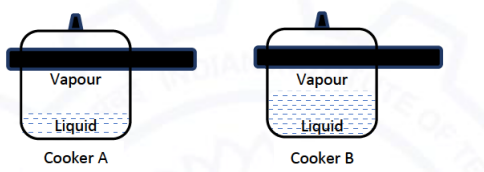
\includegraphics[width=0.5\columnwidth]{figs/fig31.png}
      \caption{}
      \label{fig:placeholder}
  \end{figure}

\hfill[GATE XE 2021]

\begin{multicols}{2}
\begin{enumerate}
    \item $g_{v,A} > g_{l,B}$
    \item $g_{v,A} < g_{l,B}$
    \item $g_{v,A} = g_{l,B}$
    \item $g_{l,B} = 2 g_{l,A}$
\end{enumerate}
\end{multicols}

\item Four different Entropy $(S)$–Temperature $(T)$ diagrams, representing liquid to vapour phase transition process of a pure substance in a closed system under constant pressure are shown. The diagram, which correctly represents the process, is:

\begin{figure}[H]
      \centering
      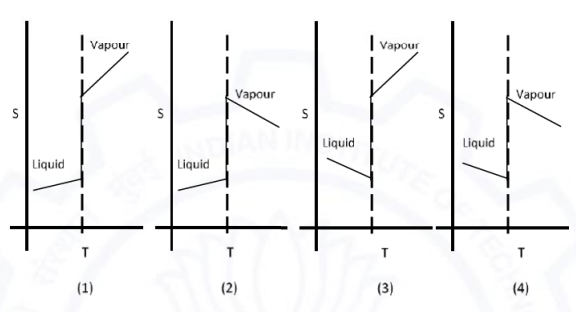
\includegraphics[width=0.5\columnwidth]{figs/fig32.png}
      \caption{}
      \label{fig:placeholder}
  \end{figure}

\hfill[GATE XE 2021]

\begin{multicols}{4}
\begin{enumerate}
\item 1
\item 2
\item 3
\item 4
\end{enumerate}
\end{multicols}

\item Air having a mass flow rate of $2\ \text{kg/s}$ enters a diffuser at $100\ \text{kPa}$ and $30^\degree$C, with a velocity of $200\ \text{m/s}$. Exit area of the diffuser is $400\ \text{cm}^2$ while the exit temperature of the air is $45^\degree$C. The rate of heat loss from the diffuser to the surrounding is $8\ \text{kJ/s}$. The pressure at the diffuser exit is \rule{3cm}{0.15mm} kPa (2 decimal places).  

For air, the characteristic gas constant is $287\ \text{J/(kgK)}$ and specific heat capacity at constant pressure is $1005\ \text{J/(kgK)}$. Assume air to be an ideal gas and the flow in the diffuser is steady.

\hfill[GATE XE 2021]


\item For the Refrigerant R-134 (at $1\ \text{MPa}$ and $50^\degree$C), the difference between the specific volume computed by assuming it to be an ideal gas and its actual specific volume is $V_{ideal} - V_{actual} = 4.529 \times 10^{-3}\ \text{m}^3/\text{kg}$. If the compressibility factor associated with this state is $Z=0.84$, then $V_{igm} - V_{actual} =$ \rule{3cm}{0.15mm} $\times 10^{-3}\ \text{m}^3/\text{kg}$ (3 decimal places).  

Here $V_{igm}$ is the specific volume calculated using the compressibility factor.  

For Refrigerant R-134 (at $1\ \text{MPa}$ and $50^\degree$C):  
The characteristic gas constant: $0.0815\ \text{kJ/(kgK)}$.  
The critical pressure and temperature are, respectively, $P_c=4.059\ \text{MPa}$ and $T_c=374.2\ \text{K}$.

\hfill[GATE XE 2021]


\item A mixture of air and water vapour enters a steady-flow adiabatic saturator at $50^\degree$C and $100\ \text{kPa}$. It leaves the saturator in a completely saturated state at temperature of $25^\degree$C and pressure of $100\ \text{kPa}$. Liquid water enters the saturator at $25^\degree$C. If air is considered to be an ideal gas, with constant specific heat capacity, the relative humidity of the air entering the saturator is \rule{3cm}{0.15mm}\% (1 decimal place).  

Use the following data:  

At $25^\degree$C: $h_f=104.87\ \text{kJ/kg}$, $h_g=2547.17\ \text{kJ/kg}$, $P_{sat}=3.161\ \text{kPa}$  

At $50^\degree$C: $h_f=209.31\ \text{kJ/kg}$, $h_g=2592.06\ \text{kJ/kg}$, $P_{sat}=12.335\ \text{kPa}$  

Specific heat capacity of air at constant pressure $C_p=1.005\ \text{kJ/(kgK)}$

\hfill[GATE XE 2021]


\item Air at a pressure of $1\ \text{MPa}$ and $300\ \text{K}$ is flowing in a pipe. An insulated evacuated rigid tank is connected to this pipe through an insulated valve. The volume of the tank is $1\ \text{m}^3$. The valve is opened and the tank is filled with air until the pressure in the tank is $1\ \text{MPa}$. Subsequently, the valve is closed. Consider air to be an ideal gas and neglect bulk kinetic and potential energy. The final temperature of air in the tank is \rule{3cm}{0.15mm} K (1 decimal place).  

Specific heat capacity of air at constant pressure $C_p=1.005\ \text{kJ/(kgK)}$ and characteristic gas constant for air $=0.287\ \text{kJ/(kgK)}$.

\hfill[GATE XE 2021]


\item A cylinder of volume $0.1\ \text{m}^3$ is filled with $100$ mol of propane (C$_3$H$_8$) at $2\ \text{MPa}$. If propane is assumed to obey the van der Waals equation of state, then its temperature is \rule{3cm}{0.15mm} K (1 decimal place).  

The van der Waals constants for propane are: $a = 939.2\ \text{kPa}\,(\text{m}^3/\text{kmol})^2$, $b = 0.0905\ \text{m}^3/\text{kmol}$.  
The universal gas constant is $8.3145\ \text{J/(mol K)}$.

\hfill[GATE XE 2021]


\item A frictionless piston cylinder device contains $1\ \text{kg}$ of an ideal gas. The gas is compressed according to $pv^{1.2} = \text{constant}$ (where $p$ is pressure and $v$ is mass specific volume), from $100\ \text{kPa}$, $250\ \text{K}$, till it reaches a temperature of $500\ \text{K}$. The heat transfer from the piston cylinder device to its surroundings is \rule{3cm}{0.15mm} kJ (2 decimal places).  

The characteristic gas constant is $287\ \text{J/(kgK)}$ and the ratio of specific heat capacities is $1.4$.

\hfill[GATE XE 2021]


\item A $0.8\ \text{m}^3$ insulated rigid tank contains $1.5\ \text{kg}$ of an ideal gas at $100\ \text{kPa}$. Electric work is done on the system until the pressure in the tank rises to $135\ \text{kPa}$. The loss in availability (exergy) associated with the process is \rule{3cm}{0.15mm} kJ (2 decimal places).  

For the ideal gas, the characteristic gas constant is $188.9\ \text{J/(kgK)}$ and the specific heat capacity at constant volume is $680\ \text{J/(kgK)}$. The temperature of the dead state is $298\ \text{K}$.

\hfill[GATE XE 2021]


\item A rigid tank contains $1.0\ \text{kg}$ of pure water consisting of liquid and vapour phases in equilibrium at $10\ \text{bar}$. If the liquid and vapour phase each occupies one half of the volume of the tank, then the net enthalpy of the contents of the tank is \rule{3cm}{0.15mm} kJ (1 decimal place).  

For saturated liquid and vapour at $10\ \text{bar}$, the thermodynamic data table provides the following values:  
$v_f=1.127\times 10^{-3}\ \text{m}^3/\text{kg}$, $v_g=194.3\times 10^{-3}\ \text{m}^3/\text{kg}$,  
$h_f=762.6\ \text{kJ/kg}$, $h_g=2776.2\ \text{kJ/kg}$.

\hfill[GATE XE 2021]


\item An air-standard Diesel cycle with a compression ratio of 16 takes air at $1\ \text{bar}$ and $300\ \text{K}$. If the maximum temperature in the cycle is $2100\ \text{K}$, then the thermal efficiency of the cycle is \rule{3cm}{0.15mm}\% (1 decimal place).  

The ratio of the specific heat capacities of air is 1.4.

\hfill[GATE XE 2021]

\item Linear low density polyethylene (LLDPE) is a copolymer of ethylene and a small fraction of \rule{2cm}{0.15mm}.

\hfill[GATE XE 2021]

\begin{multicols}{2} % Adjust number of columns as needed
    \begin{enumerate}
        \item butadiene
        \item isoprene
        \item butene
        \item hexadiene
    \end{enumerate}
\end{multicols}

\item Binary polymer blends of polypropylene and polyamide 6 are immiscible. From a thermodynamic viewpoint this is due to \rule{2cm}{0.15mm}.

\hfill[GATE XE 2021]

\begin{multicols}{2}
    \begin{enumerate}
        \item low enthalpy of mixing
        \item high entropy of mixing
        \item high enthalpy of mixing
        \item low entropy of mixing
    \end{enumerate}
\end{multicols}

\item Which one of the following is an elastomer?

\hfill[GATE XE 2021]

\begin{multicols}{2}
    \begin{enumerate}
        \item Polyamide 6,6
        \item Poly(ethylene terephthalate)
        \item Vulcanized polybutadiene
        \item High density polyethylene
    \end{enumerate}
\end{multicols}

\item Compression moulded isotropic polypropylene film exhibits in X-ray diffraction analysis

\hfill[GATE XE 2021]

\begin{multicols}{2}
\begin{enumerate}
\item Spot pattern
\item Circular ring pattern
\item Circular ring and spot pattern
\item Arc pattern
\end{enumerate}
\end{multicols}


\item Which one of the following is an example of a biodegradable polymer?

\hfill[GATE XE 2021]

\begin{multicols}{2}
\begin{enumerate}
\item Polyethylene
\item Polyamide 6,6
\item Polypropylene
\item Polylactic acid
\end{enumerate}
\end{multicols}


\item Polymer crystals show a range of melting points in contrast to single melting point of crystals of small molecules, because

\hfill[GATE XE 2021]

\begin{multicols}{2}
\begin{enumerate}
\item there is an absence of intermolecular interactions
\item there is an absence of long range ordering
\item the polymer chains are not in thermodynamic equilibrium in a metastable state
\item the melting behavior of polymer crystal is independent of sample thermal history
\end{enumerate}
\end{multicols}


\item When the rate of cooling is increased during the solidification process, the glass transition temperature of a polymer

\hfill[GATE XE 2021]

\begin{multicols}{2}
\begin{enumerate}
\item increases
\item decreases
\item stays unaltered
\item shows a non-monotonic dependence
\end{enumerate}
\end{multicols}


\item Equal and opposite forces of a constant magnitude $F$ are applied at the two ends of a thin elastomeric rod, which is held at a temperature $T_1$ ($T_g < T_1 < T_m$), where $T_g$ and $T_m$ are the glass transition temperature and melting temperature respectively. If the temperature is increased to $T_2$ ($T_g < T_2 < T_m$ and $T_2 > T_1$), the rod will

\hfill[GATE XE 2021]

\begin{multicols}{2}
\begin{enumerate}
\item expand along the loading direction and the transverse direction
\item shrink along the loading direction
\item remain dimensionally unaltered
\item expand only along the loading direction
\end{enumerate}
\end{multicols}
\item The size of a coiled polymer chain in a dilute solution is $R_G$ in a good solvent, $R_I$ in an ideal solvent and $R_P$ in a poor solvent. Select the correct ordering of sizes.

\hfill[GATE XE 2021]

\begin{multicols}{2} % Use 2 columns for the options
\begin{enumerate}[label=(\Alph*)] % Use (A), (B), etc. for labels
    \item $R_G > R_I > R_P$
    \item $R_G < R_I < R_P$
    \item $R_P > R_G > R_I$
    \item $R_P < R_G < R_I$
\end{enumerate}
\end{multicols}

\item Match the Additive to its Function.  

\begin{center}
\begin{tabular}{p{6cm} p{6cm}}
P. Tritolyl phosphate & 1. Coupling Agent \\
Q. Stearic acid       & 2. Lubricant \\
R. Silane             & 3. Plasticizer \\
S. 4-Methyl-2,6-di-t-butyl phenol & 4. Blowing Agent \\
\end{tabular}
\end{center}

\hfill[GATE XE 2021]

\begin{multicols}{2}
\begin{enumerate}
\item P–3, Q–2, R–1, S–4
\item P–3, Q–1, R–4, S–2
\item P–4, Q–1, R–3, S–2
\item P–1, Q–2, R–4, S–3
\end{enumerate}
\end{multicols}


\item Match the polymer processing operation with respect to its typical range of shear rate.  

\begin{center}
\begin{tabular}{p{6cm} p{6cm}}
P. Injection moulding & 1. $10^5$–$10^6\ \text{s}^{-1}$ \\
Q. Extrusion          & 2. $10^2$–$10^3\ \text{s}^{-1}$ \\
R. Blow moulding      & 3. $10$–$10^2\ \text{s}^{-1}$ \\
S. Compression moulding & 4. $10^3$–$10^4\ \text{s}^{-1}$ \\
\end{tabular}
\end{center}

\hfill[GATE XE 2021]

\begin{multicols}{2}
\begin{enumerate}
\item P–3, Q–4, R–2, S–1
\item P–1, Q–3, R–2, S–4
\item P–2, Q–4, R–3, S–1
\item P–3, Q–2, R–1, S–4
\end{enumerate}
\end{multicols}


\item Shear stress $(\sigma)$ and shear viscosity $(\eta)$ are plotted as functions of the shear rate $\dot{\gamma}$ for idealized “solid-like with yielding (1)” and “liquid-like (2)” materials. Associate the shear stress and viscosity plots with the appropriate material responses.

\begin{figure}[H]
      \centering
      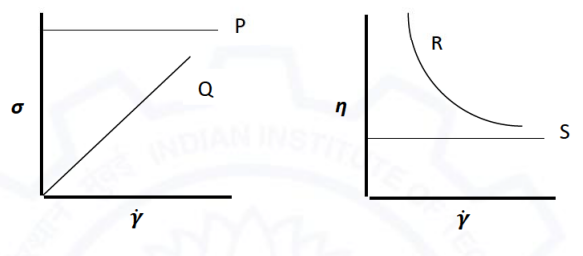
\includegraphics[width=0.5\columnwidth]{figs/fig33.png}
      \caption{}
      \label{fig:placeholder}
  \end{figure}

\hfill[GATE XE 2021]

\begin{multicols}{2}
\begin{enumerate}
\item P–2, Q–1, R–2, S–1
\item P–1, Q–2, R–1, S–2
\item P–1, Q–2, R–2, S–1
\item P–2, Q–1, R–1, S–2
\end{enumerate}
\end{multicols}


\item The plateau modulus of polystyrene has a value of $0.2\times10^6$ Pa at $150^\degree$C. Given: density of polystyrene $=1.05\ \text{g/cm}^3$, universal gas constant $R=8.3\ \text{J/(K mol)}$, and monomer molecular weight $=104\ \text{g/mol}$. The molecular weight between entanglements (rounded off to the nearest integer) of polystyrene chains is \rule{3cm}{0.15mm} g/mol.

\hfill[GATE XE 2021]


\item A unidirectional composite of epoxy and carbon fiber of 50\% by volume is made. The elastic modulus of epoxy and carbon fiber are 3.5 GPa and 350 GPa, respectively. The ratio (rounded off to one decimal place) of the modulus of the composite to the matrix modulus is \rule{3cm}{0.15mm}.

\hfill[GATE XE 2021]


\item A single screw extruder is operating at a rotational speed of 2 revolutions per second for the extrusion of a Newtonian polymer under open-discharge conditions (in absence of a die, $\Delta p=0$). The extruder has a screw diameter $D=5$ cm, a channel depth $H=0.4$ cm, distance between flights $W=1$ cm, and a helix angle $\phi=20^\degree$. Assume $\pi=3.14$. The volumetric flow rate (rounded off to 2 decimal places) is \rule{3cm}{0.15mm} cm$^3$/s.

\hfill[GATE XE 2021]


\item At $215^\degree$C, the viscosity of a polystyrene of molecular weight $250\times10^3$ g/mol is $8.0\times10^3$ Pa·s. The critical molecular weight of polystyrene is $M_c=35\times10^3$ g/mol. For a similar polystyrene of molecular weight $500\times10^3$ g/mol, the viscosity (rounded off to nearest integer) will be \rule{3cm}{0.15mm} $\times10^3$ Pa·s.

\hfill[GATE XE 2021]


\item There are two different PTFE polymer specimens of the following density $(\rho)$ and \% crystallinity. For PTFE specimen-1: $\rho=2.144\ \text{g/cm}^3$, crystallinity = 50\%. For PTFE specimen-2: $\rho=2.215\ \text{g/cm}^3$, crystallinity = 75\%. Assuming the polymer is pure and defect free, the density (rounded off to 3 decimal places) of 100\% amorphous PTFE specimen will be \rule{3cm}{0.15mm} g/cm$^3$.

\hfill[GATE XE 2021]


\item The behavior of a polymer is described by a Maxwell model consisting of a spring element of modulus $10^6$ Pa in series with a dashpot of viscosity $10^7$ Pa·s. In the solid, 50 s after the sudden application of a fixed strain of 1\%, the stress (rounded off to 2 decimal places) will be \rule{3cm}{0.15mm} $\times10^7$ Pa.

\hfill[GATE XE 2021]


\item A particular free radical polymerization process yields a polymer with a number-averaged degree of polymerization, $\bar{X}_n=100$. The monomer concentration is doubled and the initiator concentration is increased by four times. Assuming that all rate coefficients and other parameters remain unchanged, the value of $\bar{X}_n$ (rounded off to the nearest integer) is \rule{3cm}{0.15mm}.

\hfill[GATE XE 2021]


\item A polymer is synthesized from 2 moles of terephthalic acid (molecular weight of repeat unit $-O\!C\!C_6H_4CO-$ is 132 g/mol), 1 mol of ethylene glycol (repeat unit $-OCH_2CH_2O-$, 60 g/mol), and 1 mol of butylene glycol (repeat unit $-O(CH_2)_4O-$, 88 g/mol). The reaction is terminated at 99\% conversion of the acid. The number-averaged molecular weight $M_n$ (rounded off to the nearest integer) is \rule{3cm}{0.15mm} g/mol.

\hfill[GATE XE 2021]


\item A sample of natural rubber (cis-1,4-polyisoprene) is vulcanized such that one of every 240 chain carbon atoms is cross-linked. The formula unit of isoprene monomer is C$_5$H$_8$ (molecular weight = 68 g/mol). The average molecular weight (rounded off to the nearest integer) between cross-links is \rule{3cm}{0.15mm} g/mol.

\hfill[GATE XE 2021]


\item A sample of an oriented semi-crystalline polymer is subjected to uniaxial tensile stress $\sigma$ in an X-ray diffractometer. The wavelength of X-ray radiation (Cu K$\alpha$) is $\lambda=1.542$ Å. The position of the (002) peak, which was found initially at a Bragg angle of $37.50^\degree$ at $\sigma=0$ MPa, shifted to $37.45^\degree$ at $\sigma=160$ MPa. Assuming elastic deformation, the strain (rounded off to three decimal places) in the sample along the direction of applied stress is \rule{3cm}{0.15mm} $\times10^{-3}$.

\hfill[GATE XE 2021]

\item In a typical bacterial growth curve, the first order kinetics for growth rate is observed in

\hfill[GATE XE 2021]

\begin{multicols}{2}
\begin{enumerate}
\item Lag phase
\item Log phase
\item Stationary phase
\item Death phase
\end{enumerate}
\end{multicols}


\item Which one of the following microorganisms is NOT a causative agent for food borne diseases?

\hfill[GATE XE 2021]

\begin{multicols}{2}
\begin{enumerate}
\item \textit{Campylobacter jejuni}
\item \textit{Clostridium perfringens}
\item Norovirus
\item \textit{Borrelia burgdorferi}
\end{enumerate}
\end{multicols}


\item Which of the following is NOT a fermented food product?

\hfill[GATE XE 2021]

\begin{multicols}{2}
\begin{enumerate}
\item Tofu
\item Vinegar
\item Sauerkraut
\item Tempeh
\end{enumerate}
\end{multicols}


\item The Protein Efficiency Ratio (PER) is defined as

\hfill[GATE XE 2021]

\begin{multicols}{2}
\begin{enumerate}
\item Percentage of absorbed nitrogen retained in the body
\item Weight gain in body mass (in gram) per gram protein intake
\item Ratio of essential and non-essential amino acids in a protein
\item Percent \textit{in vitro} digestibility of a protein
\end{enumerate}
\end{multicols}


\item Which one of the following enzymes sequentially releases maltose from starch?

\hfill[GATE XE 2021]

\begin{multicols}{2}
\begin{enumerate}
\item \text alpha-amylase
\item \text beta-amylase
\item Glucoamylase
\item Isoamylase
\end{enumerate}
\end{multicols}


\item Which one of the following enzymes is involved in proteolysis of casein in cheese during aging?

\hfill[GATE XE 2021]

\begin{multicols}{2}
\begin{enumerate}
\item Lipase
\item Alliinase
\item Cathepsin
\item Rennin
\end{enumerate}
\end{multicols}


\item Which one of the following compounds is present in soybean and acts as phytoestrogen?

\hfill[GATE XE 2021]

\begin{multicols}{2}
\begin{enumerate}
\item Tangeretin
\item Lutein
\item Quercetin
\item Genistein
\end{enumerate}
\end{multicols}

 \item Ultra high temperature (UHT) process of pasteurization of milk is achieved by Heating at
\begin{multicols}{2}
\begin{enumerate}
    \item 145$^\degree$F for 30 minutes
    \item 161$^\degree$F for 15 seconds
    \item 280$^\degree$F for 2 seconds
    \item 400$^\degree$F for 15 seconds
\end{enumerate}
\end{multicols}

\item Bittering agent in grape fruit formed after juice extraction under acidic conditions is
\begin{multicols}{2}
\begin{enumerate}
    \item Quinine
    \item Theobromine
    \item Isohumulone
    \item Limonin
\end{enumerate}
\end{multicols}

\item The conversion of pyruvate to lactic acid in homolactic fermentation is catalyzed by

\hfill[GATE XE 2021]

\begin{multicols}{2}
\begin{enumerate}
\item Lactate dehydrogenase
\item Pyruvate dehydrogenase
\item Lactase
\item Pyruvate decarboxylase
\end{enumerate}
\end{multicols}


\item Which one of the following statements is INCORRECT with respect to Controlled Atmosphere Package (CAP) and Modified Atmosphere Package (MAP) of agro-produce?

\hfill[GATE XE 2021]


\begin{enumerate}
\item CAP and MAP limit microbial as well as biochemical activities
\item Gas composition inside a MAP during the storage is continuously monitored and regulated
\item CAP implies a greater degree of precision than MAP in maintaining specific levels of the gas composition
\item Modification of the atmosphere inside a MAP is achieved by natural interplay between respiration of products and permeation of gases through the packaging film
\end{enumerate}



\item Match unit operation in Column I with its application in food processing in Column II.

\begin{center}
\begin{tabular}{p{6cm} p{6cm}}
\textbf{Column I} & \textbf{Column II} \\
P. Hydrogenation & 1. Removal of soft wax \\
Q. Blanching & 2. Shortening of fat \\
R. Leaching & 3. Inactivation of enzyme \\
S. Winterization & 4. Separation of dye \\
\end{tabular}
\end{center}

\hfill[GATE XE 2021]

\begin{multicols}{2}
\begin{enumerate}
\item P–2, Q–4, R–2, S–1
\item P–2, Q–3, R–4, S–1
\item P–4, Q–1, R–2, S–3
\item P–4, Q–2, R–1, S–3
\end{enumerate}
\end{multicols}
\item Which of the followings are correct pair of GRAS chemical food preservative, affected organism and given food matrix?

\hfill[GATE XE 2021]

\begin{multicols}{2}
\begin{enumerate}
\item Sodium lactate – Bacteria – Pre-cooked meats
\item Caprylic acid – Insects – Cheese wraps
\item Dehydroacetic acid – Molds – Squash
\item Sodium nitrite – Clostridia – Meat curing preparations
\end{enumerate}
\end{multicols}


\item Choose the correct pair of pigment and their corresponding color in given plant product.

\hfill[GATE XE 2021]

\begin{multicols}{2}
\begin{enumerate}
\item Carotene – Yellow-orange – Peppers
\item Betanin – Purple/red – Cactus pear
\item Lycopene – Red – Red beets
\item Flavanols – Orange – Cauliflower
\end{enumerate}
\end{multicols}


\item Which of the following compounds act as anti-nutritional factors?

\hfill[GATE XE 2021]

\begin{multicols}{2}
\begin{enumerate}
\item Isoflavones
\item Trypsin Inhibitor
\item Resveratrol
\item Tannins
\end{enumerate}
\end{multicols}


\item Which of the followings is/are commonly used medium/media in the supercritical fluid extraction of spices and tea?

\hfill[GATE XE 2021]

\begin{multicols}{2}
\begin{enumerate}
\item Water
\item Carbon dioxide
\item Dichloromethane
\item Carbon dioxide with Ethanol
\end{enumerate}
\end{multicols}


\item Which of the following expressions represent the Reynolds number of a fluid flowing through a uniform circular cross section pipe?

\hfill[GATE XE 2021]

 % Adjust number of columns as needed
\begin{enumerate}
    \item $\frac{(\text{density of the fluid}) \times (\text{average velocity of the fluid}) \times (\text{internal diameter of the pipe})}{(\text{dynamic viscosity of the fluid})}$
    \item $\frac{(\text{average velocity of the fluid}) \times (\text{internal diameter of the pipe})}{(\text{kinematic viscosity of the fluid})}$
    \item $\frac{(\text{dynamic viscosity of the fluid})}{(\text{average velocity of the fluid}) \times (\text{density of the fluid}) \times (\text{internal diameter of the pipe})}$
    \item $\frac{(\text{kinematic viscosity of the fluid})}{(\text{average velocity of the fluid}) \times (\text{internal diameter of the pipe})}$
\end{enumerate}



\item Which of the following combinations of analytical equipment, property measured and food property are correct?

\hfill[GATE XE 2021]

\begin{multicols}{2}
\begin{enumerate}
\item Particle size analyzer – Particle size distribution – Span value
\item Texture profile analyzer – Morphology – Chewiness
\item Differential scanning calorimeter – Glass transition temperature – Degree of caking
\item Capillary viscometer – Viscosity – Sensory
\end{enumerate}
\end{multicols}


\item Choose the correct pair(s) of Governing Law and corresponding application(s).

\hfill[GATE XE 2021]

\begin{multicols}{2}
\begin{enumerate}
\item Hagen–Poiseuille law – Pressure drop
\item Rittinger’s law – Vapour pressure
\item Stefan–Boltzmann law – Radiation heat transfer
\item Raoult’s law – Size reduction
\end{enumerate}
\end{multicols}


\item An orange juice sample is concentrated from 10\% to 40\% (by weight) total soluble solids in a single effect evaporator with a feed rate of 3600 kg/hr at $25^\degree$C. The evaporator operates at sufficient vacuum to allow the product moisture to evaporate at $55^\degree$C. The specific heat of both feed and concentrated juice is $4.0\ \text{kJ kg}^{-1}\,^\degree$C$^{-1}$. If enthalpy of water vapour at $55^\degree$C is $2600\ \text{kJ/kg}$, heat transfer rate through the heating surface area of the evaporator in kilowatt (in integer) will be \rule{3cm}{0.15mm}.

\hfill[GATE XE 2021]


\item Dry air is fed into a tray dryer. The percentage relative humidity of the air leaving the dryer is 60\% at $70^\degree$C and 101.35 kPa. If the saturated vapour pressure of water at $70^\degree$C is 31.2 kPa, the humidity of the air leaving the dryer in kg water per kg dry air (round off to 3 decimal places) will be \rule{3cm}{0.15mm}.  

(Given: Molecular weight of water and air are 18.02 g/mol and 28.97 g/mol, respectively.)

\hfill[GATE XE 2021]


\item In a cold storage plant, 5000 kg potato having a constant specific heat capacity of $3.65\ \text{kJ kg}^{-1}\,^\degree$C$^{-1}$ are cooled from $28^\degree$C to $2^\degree$C in 24 hours. The heat of respiration of potato per 24 hour is $3.12\ \text{kJ/kg}$ during the storage. Assuming the efficiency of the storage plant to be 70\%, the capacity of the plant in ton of refrigeration (round off to 2 decimal places) is \rule{3cm}{0.15mm}.  

(Given: 1 ton of refrigeration = 3.517 kilowatt)

\hfill[GATE XE 2021]

\item Western Boundary Current in the ocean is primarily due to

\hfill[GATE XE 2021]

\begin{multicols}{2}
\begin{enumerate}
\item Ekman pumping
\item Rotation of the earth
\item River water forcing
\item Ocean floor topography
\end{enumerate}
\end{multicols}


\item The relevant non-dimensional number in deciding deepening of the thermocline driven by instability of ocean currents is

\hfill[GATE XE 2021]

\begin{multicols}{2}
\begin{enumerate}
\item Rossby number
\item Reynolds number
\item Richardson number
\item Ekman number
\end{enumerate}
\end{multicols}


\item During July–August, the highest number of monsoon low pressure systems form over

\hfill[GATE XE 2021]

\begin{multicols}{2}
\begin{enumerate}
\item Arabian Sea
\item Bay of Bengal
\item South India
\item Himalayan foothills
\end{enumerate}
\end{multicols}


\item CO$_2$ concentration in the Earth’s atmosphere is increasing because 50\% of the annual anthropogenic emissions are retained in the atmosphere. If nations agree to reduce annual CO$_2$ emissions by one Giga ton every year starting from 2021, then in which year will the CO$_2$ concentration in the atmosphere stop rising due to anthropogenic emissions?  

Take the anthropogenic CO$_2$ emissions in 2020 as 40 Giga tons.

\hfill[GATE XE 2021]

\begin{multicols}{2}
\begin{enumerate}
\item 2020
\item 2050
\item 2060
\item 2100
\end{enumerate}
\end{multicols}


\item The figure shows a schematic of Indian Ocean surface circulation. This pattern is representative of the circulation in which month of the year?

\begin{figure}[H]
      \centering
      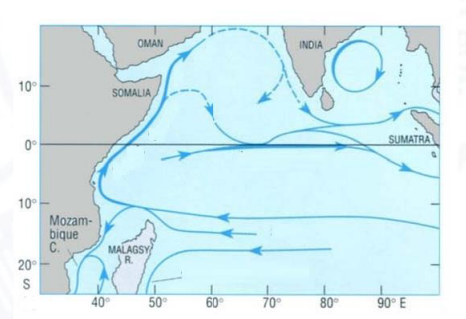
\includegraphics[width=0.5\columnwidth]{figs/fig34.png}
      \caption{}
      \label{fig:placeholder}
  \end{figure}

\hfill[GATE XE 2021]

\begin{multicols}{2}
\begin{enumerate}
\item January
\item July
\item May
\item November
\end{enumerate}
\end{multicols}


\item Over the open ocean, if the air–sea temperature difference is zero, then which of the following statements is/are always true?

\hfill[GATE XE 2021]

\begin{multicols}{2}
\begin{enumerate}
\item Sensible heat flux is zero
\item Latent heat flux is zero
\item Momentum flux is zero
\item Net energy flux is zero
\end{enumerate}
\end{multicols}


\item The psychrometric equation, which is useful in measuring humidity, is derived assuming the following process(es).

\hfill[GATE XE 2021]

\begin{multicols}{2}
\begin{enumerate}
\item Isobaric process
\item Isothermal process
\item Adiabatic process
\item Isentropic process
\end{enumerate}
\end{multicols}

\item The water vapour mixing ratio of an air parcel increases from 10 g/kg to 20 g/kg at a constant pressure of 1010 hPa and temperature of 300 K. The change in virtual temperature is \rule{3cm}{0.15mm} K (to one decimal place).

\hfill[GATE XE 2021]


\item The Ekman layer thickness, if turbulent diffusivity is 0.01 m$^2$/s, is \rule{3cm}{0.15mm} m. Take Coriolis parameter to be $10^{-4}$ s$^{-1}$. (Round off to the nearest integer).

\hfill[GATE XE 2021]


\item The figure shows vertical variation of two chemicals P and Q measured in the Pacific Ocean. Identify the correct combination showing (P, Q) pair from the list below.

\begin{figure}[H]
      \centering
      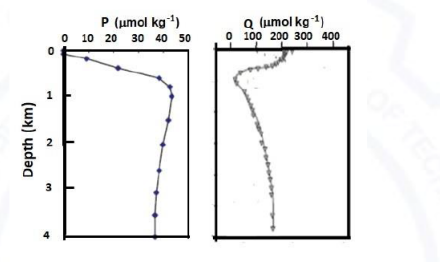
\includegraphics[width=0.5\columnwidth]{figs/fig35.png}
      \caption{}
      \label{fig:placeholder}
  \end{figure}

\hfill[GATE XE 2021]

\begin{multicols}{2}
\begin{enumerate}
\item Oxygen, Nitrate
\item Oxygen, Neon
\item Nitrate, Oxygen
\item Neon, Nitrate
\end{enumerate}
\end{multicols}


\item Consider tropical high-level clouds and low-level stratus clouds with bases at 12 km and 1 km above the surface of the Earth, respectively. Which of the following statement(s) is/are correct?

\hfill[GATE XE 2021]

\begin{multicols}{2}
\begin{enumerate}
\item High clouds are composed of ice crystals
\item High clouds have a larger albedo than low clouds
\item High clouds have a net warming effect on climate
\item Low clouds have a net warming effect on climate
\end{enumerate}
\end{multicols}


\item Which of the following statement(s) is/are correct in the context of Sverdrup transport?

\hfill[GATE XE 2021]

\begin{multicols}{2}
\begin{enumerate}
\item Sverdrup transport is always in the meridional direction
\item Sverdrup transport is always orthogonal to the wind direction
\item Sverdrup transport depends on the variation of the Coriolis parameter
\item Sverdrup transport is only due to ageostrophic currents
\end{enumerate}
\end{multicols}
\item Which of the following statement(s) is/are correct regarding the Hadley cell?

\hfill[GATE XE 2021]

\begin{multicols}{2}
\begin{enumerate}
\item The ascending branch is narrower than its descending branch
\item Thunderstorms are more frequent in the subsiding region of the Hadley cell than in its ascending region
\item The lower level winds between the ascending and descending branches of the Hadley cell are north-westerly
\item Latent heat is transported from the subsiding to the ascending region of the Hadley cell
\end{enumerate}
\end{multicols}


\item Which of the following statement(s) is/are true about the ocean circulation?

\hfill[GATE XE 2021]

\begin{multicols}{2}
\begin{enumerate}
\item Large-scale ocean surface currents are driven by winds
\item Cold, dense and salty water forms in the North Atlantic Ocean
\item Upwelling currents bring warm nutrient-deficient water to the surface of the ocean
\item Thermohaline circulation does not transport energy in the meridional direction
\end{enumerate}
\end{multicols}


\item Coral reefs are found primarily in tropical and subtropical shallow seawaters. Which of the following statement(s) is/are correct?

\hfill[GATE XE 2021]

\begin{multicols}{2}
\begin{enumerate}
\item Corals require plenty of sunlight for photosynthesis and sunlight is abundant in the tropical and subtropical latitudes
\item Corals grow optimally in seawater unsaturated in carbonate, which is found only in the tropical and subtropical oceans
\item Corals grow optimally in fresh low-salinity water
\item Corals grow optimally in water temperatures between 23$^\degree$C and 29$^\degree$C
\end{enumerate}
\end{multicols}


\item In an incompressible fluid, the horizontal divergence is $-0.01\ \text{s}^{-1}$. Then, the vertical velocity at 50 m above a flat surface is \rule{3cm}{0.15mm} m/s. (Round off to one decimal place)

\hfill[GATE XE 2021]


\item In an atmosphere, temperature $T$ decreases linearly with height above the ground ($z$), i.e., $T(z) = T_0 - \gamma z$, where $\gamma$ is a constant. Surface pressure is 900 hPa. If the atmosphere is at rest, then the value of $z$ at which the pressure decreases to half of that at the surface is \rule{3cm}{0.15mm} m (round off to nearest integer).  

Take acceleration due to gravity $g = 10\ \text{m/s}^2$, gas constant $R = 300\ \text{J/(kg K)}$, $T_0 = 300\ \text{K}$ and $\gamma = 1/30\ \text{K/m}$. Assume atmosphere behaves as an ideal gas.

\hfill[GATE XE 2021]


\item In a local Cartesian system, a zonal jet has a form $u(y) = u_0 \brak{1 - \dfrac{y^2}{L^2}}$, for $-L<y<L$. Here, $y$ is the meridional distance measured from the axis of the jet and is positive northward. The vertical component of vorticity of this flow at $y=L/2$ is \rule{3cm}{0.15mm} s$^{-1}$. (Round off to 3 decimal places)  

Take $u_0 = 50\ \text{m/s}$ and $L = 5$ km.

\hfill[GATE XE 2021]


\item An eastward flow with a speed of 10 m/s goes from station M to station N, which are separated by a distance of 1 km. The temperature at station N is always higher than that at station M by 10 K. The absolute change in temperature due to advection at the mid-point between the stations in 50 s is \rule{3cm}{0.15mm} K (round off to nearest integer).

\hfill[GATE XE 2021]


\item Suppose, because of the doubling of atmospheric CO$_2$ concentration, an ocean water column receives an additional net energy input of 4 W/m$^2$. If the entire water column of depth 1 km heats up uniformly, the water temperature will increase by 1 K in \rule{3cm}{0.15mm} years (round off to nearest integer).  

Assume all the additional heat added is retained and not lost. Take density of seawater = 1000 kg/m$^3$; specific heat capacity of seawater = 4200 J/(kg K).

\hfill[GATE XE 2021]


\item Consider a layer of atmosphere between 5 and 6 km height. The downwelling longwave radiation at 5 and 6 km is 240 and 230 W/m$^2$, respectively. The upwelling longwave radiation at these heights is 260 and 240 W/m$^2$, respectively. The longwave heating rate in this layer is \rule{3cm}{0.15mm} K/day. (Round off to one decimal place)  

Take the average density of air in this layer to be 0.5 kg/m$^3$; specific heat capacity of air at constant pressure = 1000 J/(kg K).

\hfill[GATE XE 2021]


\item A spherical asteroid, revolving around the Sun in a circular orbit, is in radiative balance. Suddenly, the asteroid enters the shadow of a planet and solar radiation is cut off. Assuming that the asteroid emits as a blackbody in the longwave regime, the time taken to reduce the average temperature of the asteroid by 0.5 K is \rule{3cm}{0.15mm} seconds (round off to nearest integer).  

Ignore the temporal change in radiation emitted by the asteroid during this cooling period.  

The physical properties of the asteroid are: diameter = 2 m, density = 3000 kg/m$^3$, specific heat = 2000 J/(kg K), albedo = 0.8 in shortwave radiation. Take solar constant = 500 W/m$^2$, Stefan–Boltzmann constant = $5.67 \times 10^{-8}$ W m$^{-2}$ K$^{-4}$.

\hfill[GATE XE 2021]

\end{enumerate}

\end{document}















\end{document}
